




Probability is the art of reasoning precisely about uncertainty. Starting from a small collection of axioms, we will build up a theory that lets us make (often surprisingly strong) quantitative statements about randomness -- from coin tosses and card shuffles all the way up to random walks, branching processes and the celebrated central limit theorem. One of the joys of the subject is how far a few simple ideas (independence, expectation, indicators, generating functions) can be pushed, and we will try to emphasise these recurring techniques throughout.

This article constitutes my notes for the `Probability' course, held in Lent 2021 at Cambridge. These notes are \emph{not a transcription of the lectures}, and differ significantly in quite a few areas. Still, all lectured material should be covered.



\section{Setting Up Probability}

We are going to build up probability from the very basic axioms. This will give us a firm mathematical basis to work from, but also will match the intuitive notions of probability that you have hopefully developed before reading this handout.

\subsection{Probability Spaces}

The basic object of study in probability theory is that of \emph{probability spaces}. We begin by defining how we can talk about the idea of `events' formally. What we want from our definition will be some way to have a set of possible `outcomes' (a \emph{sample space}), from which we can combine different outcomes to form various `events'. This leads almost directly to the definition of an \emph{event space}.

\begin{definition}[Event Space] The collection $\FF$ of subsets of the sample space $\Omega$ is an \vocab{event space} or \vocab{$\sigma$-algebra} if
	\begin{enumerate}
		\item $\FF$ is non-empty,
		\item if $A \in \FF$, then $\Omega \backslash A \in \FF$,
		\item if $A_1, A_2, \dots \in \FF$, then $\bigcup_{i = 1}^{\infty} A_i \in \FF$.
	\end{enumerate}
\end{definition}

Within this system, $A \cup B$ corresponds to either $A$ or $B$ occurring, $A \cap B$ corresponds to both $A$ and $B$ occurring, and $\Omega \backslash A$ corresponds with anything but $A$ occurring. You get the idea.

Our main goal in the study of probability is to assign some sort of `likelihood' to events in the event space. This is done through the introduction of a \emph{probability measure}.


\begin{definition}[Probability Measure]
	We say that a function $\PP : \FF \rightarrow \R$ is a \vocab{probability measure} on $(\Omega, \FF)$ if
	\begin{enumerate}
		\item $\PP(A) \geq 0$ for all $A \in \FF$,
		\item $\PP(\Omega) = 1$,
		\item if $A_1, A_2, \dots$ are disjoint events in $\FF$, then $\PP\left(\bigcup_{i = 1}^{\infty} A_i\right) = \sum_{i = 1}^{\infty} \PP(A_i)$.
	\end{enumerate} 
\end{definition}

These properties of the probability measure should match your own intuition about the way that probability works. Putting all the pieces together, we get our main object of study: the \emph{probability space}.

\begin{definition}[Probability Space]
	A \vocab{probability space} is a triple $(\Omega, \FF, \PP)$ such that $\Omega$ is non empty, $\FF$ is an event space on $\Omega$, and $\PP$ is a probability measure on $(\Omega, \FF)$.
\end{definition}


If we only have to deal with say finite (or even countable) $\Omega$, then it makes sense to usually take $\FF$ to just be the power set of $\Omega$. In this case, if $\Omega = \{\omega_1, \omega_2, \dots \}$, then we can construct any probability measure $\PP$ by just specifying $\PP(\{\omega_i\})$ for all $i$, as then for $A \in \FF$, we can get $\PP(A) = \sum_{\omega \in A} \PP(\{\omega\})$.

Before going any further, we should note some basic properties of probability measures, all of which follow pretty quickly from the definition.

\begin{proposition}[Properties of Probability Measures]
	Let $(\Omega, \FF, \PP)$ be a probability space, and let $A, B \in \FF$. Then
	\begin{enumerate}[label=(\roman*)]
		\item $\PP(\Omega \backslash A) = 1 - \PP(A)$,
		\item $\PP(\emptyset) = 0$,
		\item if $A \subseteq B$ then $\PP(A) \leq \PP(B)$,
		\item $\PP(A \cup B) = \PP(A) + \PP(B) - \PP(A \cap B)$.
	\end{enumerate}
\end{proposition}
\begin{proof}
	For (i), the events $A$ and $\Omega \backslash A$ are disjoint with union $\Omega$, so $\PP(A) + \PP(\Omega \backslash A) = \PP(\Omega) = 1$. Then (ii) follows by taking $A = \Omega$. For (iii), we can write $B$ as the disjoint union $B = A \cup (B \backslash A)$, so $\PP(B) = \PP(A) + \PP(B \backslash A) \geq \PP(A)$. Finally for (iv), we write $A \cup B$ as the disjoint union $A \cup (B \backslash (A \cap B))$, giving
	$$
	\PP(A \cup B) = \PP(A) + \PP(B \backslash (A \cap B)) = \PP(A) + \PP(B) - \PP(A \cap B),
	$$
	where the last step uses that $A \cap B \subseteq B$.
\end{proof}

\subsection{Classical Probability and Counting}

The setting in which probability historically began (think gambling problems in the 17th century) is what's now called \emph{classical probability}: a finite sample space in which every outcome is equally likely. That is, we take $\Omega = \{\omega_1, \dots, \omega_n\}$ and
$$
\PP(A) = \frac{|A|}{|\Omega|} \quad \text{for } A \subseteq \Omega.
$$
Computing probabilities in this setting amounts to \emph{counting}, so it is worth pausing to build up a small toolbox of combinatorial facts. We will state them briefly, since they should be mostly familiar.

\begin{fact}[Counting Toolbox]
	Let $\Omega$ be a set of $n$ elements. Then
	\begin{enumerate}[label=(\roman*)]
		\item the number of orderings (permutations) of $\Omega$ is $n! = n(n-1) \cdots 1$,
		\item the number of subsets of $\Omega$ of size $k$ is $\binom{n}{k} = \frac{n!}{k!(n - k)!}$,
		\item the number of ways to partition $\Omega$ into $k$ disjoint subsets $\Omega_1, \dots, \Omega_k$ with $|\Omega_i| = n_i$ and $n_1 + \cdots + n_k = n$ is the \vocab{multinomial coefficient}
		$$
		\binom{n}{n_1, n_2, \dots, n_k} = \binom{n}{n_1}\binom{n - n_1}{n_2} \cdots \binom{n - n_1 - \cdots - n_{k - 1}}{n_k} = \frac{n!}{n_1! \, n_2! \cdots n_k!}.
		$$
	\end{enumerate}
\end{fact}

Armed with these, let's do some classical probability. The following examples are, well, classics.

\begin{example}[Aces on Top]
	A standard deck of 52 cards is shuffled so that all $52!$ orderings are equally likely. What is the probability that the top two cards are both aces?

	We take $\Omega$ to be the set of all $52!$ orderings. The number of orderings with aces in the top two positions is $4 \times 3 \times 50!$ (choose which aces go first and second, then order the rest freely). So the probability is
	$$
	\frac{4 \cdot 3 \cdot 50!}{52!} = \frac{4 \cdot 3}{52 \cdot 51} = \frac{1}{221}.
	$$
\end{example}

\begin{example}[The Birthday Problem]
	There are $n$ people in a room. What is the probability that at least two of them share a birthday\footnote{We'll assume that there's 365 days in a year, that no one is born on the 29th of February, and that all birthdays are equally likely.}?

	Take $\Omega = \{1, \dots, 365\}^n$, with all outcomes equally likely. Let $A$ be the event that at least two birthdays coincide. It's much easier to count the complement, the event that all $n$ birthdays are distinct. There are $365 \cdot 364 \cdots (365 - n + 1)$ such outcomes, so
	$$
	\PP(A) = 1 - \frac{365 \cdot 364 \cdots (365 - n + 1)}{365^n}.
	$$
	Plugging in numbers gives a somewhat surprising result: with $n = 22$ we get $\PP(A) \approx 0.476$, and with $n = 23$ we get $\PP(A) \approx 0.507$. So in a room of just 23 people, it's more likely than not that two people share a birthday.
\end{example}

The trick of `counting the complement' used above is worth remembering -- it is frequently much easier to count the outcomes avoiding some property than those with it.

Since factorials appear all over the place in these calculations, it is quite helpful to know how fast $n!$ actually grows. The definitive answer is given by \emph{Stirling's formula}. We write $a_n \sim b_n$ to mean $a_n / b_n \rightarrow 1$ as $n \rightarrow \infty$.

\begin{theorem}[Stirling's Formula]
	As $n \rightarrow \infty$, we have
	$$
	n! \sim n^n e^{-n} \sqrt{2 \pi n}.
	$$
\end{theorem}

We will prove the following weaker statement, which is enough for many applications (it pins down $\log n!$ to first order, but not the constant $\sqrt{2\pi}$).

\begin{proposition}[Weak Stirling]
	As $n \rightarrow \infty$, $\log n! \sim n \log n$.
\end{proposition}
\begin{proof}
	Let $l_n = \log n! = \log 2 + \log 3 + \cdots + \log n$. Since $\log$ is increasing, for any integer $k$ we have $\log k \leq \log x \leq \log(k+1)$ for $x \in [k, k+1]$, and integrating over such intervals gives
	$$
	\sum_{k = 1}^{n - 1} \log k \leq \int_1^n \log x \dd x \leq \sum_{k = 2}^{n} \log k,
	$$
	that is, $l_{n - 1} \leq n \log n - n + 1 \leq l_n$. Using both bounds, for all $n$ we get
	$$
	n \log n - n + 1 \leq l_n \leq (n + 1)\log (n + 1) - n,
	$$
	and dividing through by $n \log n$ and letting $n \rightarrow \infty$ gives $l_n / (n \log n) \rightarrow 1$, as required.
\end{proof}

The proof of the full result is a little involved (the constant $\sqrt{2\pi}$ is usually extracted from the asymptotics of the central binomial coefficient $\binom{2n}{n}$, using Wallis' product), and we will not give it here. A fact worth keeping from that analysis is
$$
2^{-2n}\binom{2n}{n} \sim \frac{1}{\sqrt{\pi n}},
$$
which says that the probability of getting exactly $n$ heads in $2n$ tosses of a fair coin decays like $1/\sqrt{\pi n}$ -- slowly!

\subsection{Conditional Probability and Independence}

In our day-to-day experience, we know that knowledge about one event can influence how likely we determine another event is to occur. This type of thinking motivates the introduction of \emph{conditional probability}.

\begin{definition}[Conditional Probability]
	If $A, B \in \FF$ and $\PP(B) > 0$, the \vocab{probability of $A$ given $B$} is denoted $\PP(A \mid B)$, and is given by
	$$
	\PP(A \mid B) = \frac{\PP(A \cap B)}{\PP(B)}.
	$$
\end{definition}

It's not hard to check that $\PP(\; \cdot \mid B)$ is a probability measure, as we would expect -- it's just assigning probabilities to events in $\FF$ in a different way!

A natural thing to care about is if knowledge about an event \emph{doesn't} influence how likely another event is. We call such events independent.

\begin{definition}[Independent Events]
We say that events $A, B$ in a probability space $(\Omega, \FF, \PP)$ are \vocab{independent} if
$$
\PP(A \cap B) = \PP(A) \PP(B),
$$
and \vocab{dependent} otherwise.
\end{definition}

We can see immediately that $A, B$ independent implies that
$$
\PP(A \mid B) = \PP(A) \quad \text{and} \quad \PP(B \mid A) = \PP(B),
$$
if $\PP(A), \PP(B) \neq 0$. However, this definition is slightly more general than this property since it handles events with zero probability.
We can generalise this notion of independence to multiple events, and we get a criterion that's stronger than pairwise independence\footnote{It's not hard to construct an example of events that are pairwise independent but wouldn't be independent in any reasonable sense.}.

\begin{definition}[Mutually Independent Events]
	We say that the events $A_1$, $A_2$, $A_3$, $\dots$ are \vocab{mutually independent} if
	$$
	\PP(A_{i_1} \cap A_{i_2} \cap \cdots \cap A_{i_r}) = \PP(A_{i_1}) \PP(A_{i_2}) \cdots \PP(A_{i_r}),
	$$
	for any $i_1, i_2, \dots, i_r$ and $r \geq 2$.
\end{definition}

So if conditional probability tells us about the likelihood of a certain event in one particular scenario, then it's easy to imagine that knowing about the likelihood in every scenario would then just give you the likelihood in general. Such thinking is formalised in the \emph{law of total probability}, also known as the \emph{partition theorem}.

\begin{theorem}[Partition Theorem]
	Let $\{B_1, B_2, \dots\}$ be a collection of disjoint events such that $\PP(B_i) > 0$ for all $i$ and $\bigcup_{i = 1}^{\infty} B_i = \Omega$. Then
	$$
	\PP(A) = \sum_i \PP(A \mid B_i) \PP(B_i),
	$$
	for any $A \in \FF$.
\end{theorem}
\begin{proof}
	We can compute that
	\begin{align*}
		\sum_{i} \PP(A \mid B_i) \PP(B_i) &= \sum_i \PP(A \cap B_i) = \PP\left(\bigcup_i (A \cap B_i)\right) = \PP(A),
	\end{align*}
	as required.
\end{proof}

Using the partition theorem, we can establish the famous \vocab{Bayes' theorem}, which allows us to use knowledge about $\PP(A \mid B_j)$ to give information about $\PP(B_j \mid A)$:
$$
\PP(B_j \mid A) = \frac{\PP(A \mid B_j) \PP(B_j)}{\PP(A)} = \frac{\PP(A \mid B_j) \PP(B_j)}{\sum_i \PP(A \mid B_i) \PP(B_i)}.
$$

Bayes' theorem is the basis of essentially all of Bayesian statistics -- it lets us `reverse the direction' of conditioning, updating our beliefs about which scenario $B_j$ we are in, given that we observed $A$. It also has a habit of producing answers that clash violently with intuition, as the next example shows.

\begin{example}[False Positives]
	Suppose that $0.1\%$ of the population suffer from a certain rare condition, and that we have a test for the condition which is positive for $98\%$ of sufferers, but also (falsely) positive for $1\%$ of non-sufferers. A person is chosen at random and tests positive. What is the probability that they actually have the condition?

	Let $A$ be the event that the person has the condition, and $P$ the event that they test positive. The situation is summarised by the following tree, with the two stages of conditioning shown left to right.
	\begin{center}
	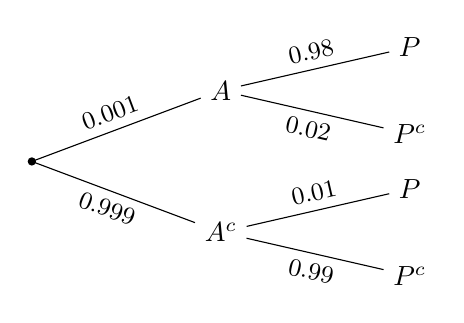
\begin{tikzpicture}[x=1cm,y=1cm]
		\coordinate (r) at (0,0);
		\node (A)  at (2.4,0.9) {$A$};
		\node (Ac) at (2.4,-0.9) {$A^c$};
		\node (AP)  at (4.8,1.45) {$P$};
		\node (APc) at (4.8,0.35) {$P^c$};
		\node (AcP)  at (4.8,-0.35) {$P$};
		\node (AcPc) at (4.8,-1.45) {$P^c$};
		\draw (r) -- (A) node [midway, above, sloped, font=\small] {$0.001$};
		\draw (r) -- (Ac) node [midway, below, sloped, font=\small] {$0.999$};
		\draw (A) -- (AP) node [midway, above, sloped, font=\small] {$0.98$};
		\draw (A) -- (APc) node [midway, below, sloped, font=\small] {$0.02$};
		\draw (Ac) -- (AcP) node [midway, above, sloped, font=\small] {$0.01$};
		\draw (Ac) -- (AcPc) node [midway, below, sloped, font=\small] {$0.99$};
		\fill (r) circle (1.5pt);
	\end{tikzpicture}
	\end{center} Then by Bayes' theorem,
	\begin{align*}
		\PP(A \mid P) &= \frac{\PP(P \mid A) \PP(A)}{\PP(P \mid A)\PP(A) + \PP(P \mid A^c) \PP(A^c)} \\
		&= \frac{0.98 \times 0.001}{0.98 \times 0.001 + 0.01 \times 0.999} \approx 0.09.
	\end{align*}
	So despite the test looking quite accurate, a positive result only means a $9\%$ chance of having the condition! The point is that the false positive rate ($1\%$) utterly dwarfs the prevalence of the condition ($0.1\%$): in a population of 1000 people, we expect about 1 true positive but about 10 false positives, so only about 1 in 11 positive tests is genuine.
\end{example}

Another recurring subtlety is that the answer to a conditional probability question depends delicately on \emph{exactly} what information you condition on.

\begin{example}[Two Children]
	I have two children. Consider the following three statements:
	\begin{enumerate}[label=(\alph*)]
		\item at least one of them is a boy;
		\item the eldest is a boy;
		\item at least one of them is a boy born on a Thursday.
	\end{enumerate}
	Given each statement in turn, what is the probability that I have two boys? (Assume boys and girls, and days of the week, are equally likely and independent.)

	Writing the sexes in age order, the equally likely possibilities are $BB, BG, GB, GG$. Given (a), we condition on $\{BB, BG, GB\}$, so
	$$
	\PP(BB \mid BB \cup BG \cup GB) = \frac{1/4}{3/4} = \frac13.
	$$
	Given (b), we condition on $\{BB, BG\}$, and the answer is $\frac12$ -- so (a) and (b) genuinely differ, even though both `tell you there's a boy'.

	For (c), splitting each boy into `born on Thursday' ($T$, probability $\frac{1}{14}$ per child) or `boy not born on Thursday' ($N$, probability $\frac{6}{14}$), a short computation with the equally likely fine-grained outcomes gives
	$$
	\PP(\text{two boys} \mid \text{at least one } T) = \frac{\frac{1}{14}\cdot\frac{1}{14} + 2\cdot\frac{1}{14}\cdot\frac{6}{14}}{\frac{1}{14}\cdot\frac{1}{14} + 2\cdot\frac{1}{14}\cdot\frac{6}{14} + 2 \cdot \frac{1}{14}\cdot\frac{7}{14}} = \frac{13}{27} \approx 0.48.
	$$
	Astonishingly, the (apparently irrelevant!) day of birth moves the answer from $\frac13$ towards $\frac12$. Intuitively, `a boy born on a Thursday' is more likely to be reportable in a two-boy family, since there are two chances for it to occur.
\end{example}

Conditioning can be genuinely subtle, and it's worth seeing one famous trap: aggregating data across dissimilar populations can \emph{reverse} the direction of an inequality between conditional probabilities.

\begin{example}[Simpson's Paradox]
	A university admits students from two types of school, and it's observed that applicants from state schools are admitted at a higher rate than applicants from independent schools \emph{both} among men and among women -- yet when the data is aggregated, independent school applicants are admitted at a higher rate overall.

	This can genuinely happen with real numbers, and there is no contradiction. Writing $A$ for admission, $C$ for coming from a state school and $B$ for being a man, the `paradoxical' data amounts to
	$$
	\PP(A \mid B \cap C) > \PP(A \mid B \cap C^c), \quad \PP(A \mid B^c \cap C) > \PP(A \mid B^c \cap C^c),
	$$
	but $\PP(A \mid C) < \PP(A \mid C^c)$. If we try to `average' the first two inequalities using the partition theorem, we find
	$$
	\PP(A \mid C) = \PP(A \mid B \cap C)\PP(B \mid C) + \PP(A \mid B^c \cap C) \PP(B^c \mid C),
	$$
	and similarly for $C^c$ -- but the weights $\PP(B \mid C)$ and $\PP(B \mid C^c)$ need not be equal! It is only when the populations are mixed in the same proportions ($\PP(B \mid C) = \PP(B \mid C^c)$) that the intuitive conclusion $\PP(A \mid C) > \PP(A \mid C^c)$ actually follows. The moral: be very careful about pooling conditional probabilities.
\end{example}

\subsection{Continuity of Probability Measures}

In the definitions for event spaces ($\sigma$-algebras) and probability measures, you may notice that we specify rules for countably infinite sequences of events. This is for good reason -- there's plenty of natural scenarios where such a setup is useful. For example, consider the experiment of tossing a coin until you get heads, in which it is possible to get an arbitrarily long run of tails before you stop tossing. To make working with such scenarios easier, we can establish a result which allows us study events as limits of a sequence of events -- that the probability measure is continuous.


\begin{definition}[Limits of Events]
	We say that a sequence of events $A_1, A_2, \dots$ is \emph{increasing} if $A_1 \subseteq A_2 \subseteq \cdots$. We define the \vocab{limit} as
	$$
	\lim_{n \to \infty} A_n = \bigcup_{n = 1}^{\infty} A_n.
	$$
\end{definition}

\begin{theorem}[Continuity of Probability Measures]
	Let $(\Omega, \FF,\PP)$ be a probability space. If $A_1, A_2, \dots$ is an increasing sequence of events in $\FF$ with limit $A$, then $\PP(A) = \lim_{n \to \infty} \PP(A_n)$.
\end{theorem}
\begin{proof}
	Define $B_i = A_i \backslash A_{i - 1}$, with $B_1 = A_1$. Then we have
	$$
A = B_1 \cup B_2 \cup B_3 \cup \cdots
	$$
	which is the union of disjoint events in $\FF$. Thus we have
	\begin{align*}
		\PP(A) &= \PP\left(\bigcup_{n = 1}^{\infty} A_n\right) = \PP\left(\bigcup_{n = 1}^{\infty} B_n\right) \\
		&= \lim_{n \to \infty} \sum_{i = 1}^{n} \PP(B_n) = \lim_{n \to \infty} \PP(B_1 \cup \cdots \cup B_n) \\ &= \lim_{n \to \infty} \PP(A_n),
	\end{align*}
	as required.
\end{proof}

As a side note, the type of construction used to define $B_i$ can be quite helpful when we want to deal with a disjoint union, rather than some non-disjoint sequence of events (since it works nicely with the definition of the probability space!)

Another rather intuitive notion is that of probabilities being `subadditive' when events are \emph{not} disjoint, which we can see in the following result.

\begin{theorem}[Boole's Inequality -- The Union Bound]
	For any sequence of events $A_1, A_2, \dots$ we have
	$$
	\PP\left(\bigcup_{i = 1}^{\infty} A_i\right) \leq \sum_{i = 1}^{\infty} \PP(A_i).
	$$
\end{theorem}
\begin{proof}
	We use a similar construction to the previous proof. Let $B_1 = A_1$, and define $B_i = A_i \backslash \bigcup_{k = 1}^{i - 1} A_k$. Then we have
	$$
	\PP\left(\bigcup_{i = 1}^{\infty} A_i\right) = \PP\left(\bigcup_{i = 1}^{\infty} B_i\right) = \sum_{i = 1}^{\infty} \PP(B_i) \leq \sum_{i = 1}^{\infty} \PP(A_i),
	$$
	where the inequality occurs since $B_i \subseteq A_i$ implies $\PP(B_i) \leq \PP(A_i)$.
\end{proof}

\subsection{Inclusion-Exclusion}

We saw earlier that $\PP(A \cup B) = \PP(A) + \PP(B) - \PP(A \cap B)$: if we just add up the two probabilities, we've double counted the overlap, so we subtract it off once. If we try the same thing with three events, adding up the pairwise corrections over-corrects for the triple overlap, and we need to add that back on:
$$
\PP(A \cup B \cup C) = \PP(A) + \PP(B) + \PP(C) - \PP(A \cap B) - \PP(B \cap C) - \PP(A \cap C) + \PP(A \cap B \cap C).
$$
Continuing this alternating pattern of corrections gives the general \emph{inclusion-exclusion formula}.

\begin{theorem}[Inclusion-Exclusion]
	Let $A_1, \dots, A_n$ be events. Then
	$$
	\PP\left(\bigcup_{i = 1}^{n} A_i\right) = \sum_{k = 1}^{n} (-1)^{k + 1} \sum_{1 \leq i_1 < \cdots < i_k \leq n} \PP(A_{i_1} \cap \cdots \cap A_{i_k}).
	$$
\end{theorem}
\begin{proof}
	We induct on $n$, with the case $n = 2$ already established. Assuming the result for $n - 1$ events, we have
	\begin{align*}
		\PP\left(\bigcup_{i = 1}^{n} A_i\right) &= \PP\left(\bigcup_{i = 1}^{n-1} A_i\right) + \PP(A_n) - \PP\left(\bigcup_{i = 1}^{n - 1} (A_i \cap A_n)\right).
	\end{align*}
	Now we apply the inductive hypothesis to both unions on the right hand side, the second with $B_i = A_i \cap A_n$. The first gives all of the terms not involving $A_n$, the term $\PP(A_n)$ gives the term involving only $A_n$, and expanding the second union gives (after noting $B_{i_1} \cap \cdots \cap B_{i_k} = A_{i_1} \cap \cdots \cap A_{i_k} \cap A_n$, and with a sign flip from the minus sign) exactly the terms involving $A_n$ and at least one other event. Collecting everything up gives the required formula.
\end{proof}

\begin{remark}
	In the classical setting where $\PP(A) = |A|/|\Omega|$, multiplying through by $|\Omega|$ gives the corresponding counting formula
	$$
	|A_1 \cup \cdots \cup A_n| = \sum_{k = 1}^{n} (-1)^{k + 1} \sum_{i_1 < \cdots < i_k} |A_{i_1} \cap \cdots \cap A_{i_k}|,
	$$
	which you may well have seen in `Numbers and Sets'.
\end{remark}

If we don't need an exact answer, we can truncate the inclusion-exclusion sum, and it's useful to know which way the truncation errs. The answer alternates: stopping after an odd number of terms overestimates, and after an even number underestimates. These are the \emph{Bonferroni inequalities}.

\begin{theorem}[Bonferroni Inequalities]
	Let $A_1, \dots, A_n$ be events and $1 \leq r \leq n$. If $r$ is odd, then
	$$
	\PP\left(\bigcup_{i = 1}^n A_i\right) \leq \sum_{k = 1}^{r} (-1)^{k + 1} \sum_{i_1 < \cdots < i_k} \PP(A_{i_1} \cap \cdots \cap A_{i_k}),
	$$
	and if $r$ is even the reverse inequality holds.
\end{theorem}
\begin{proof}
	We induct on $n$, exactly as in the proof of inclusion-exclusion (the case $n = 2$ is easy to check directly). Suppose $r$ is odd, and write
	$$
	\PP\left(\bigcup_{i = 1}^{n} A_i\right) = \PP\left(\bigcup_{i = 1}^{n-1} A_i\right) + \PP(A_n) - \PP\left(\bigcup_{i = 1}^{n - 1} B_i\right),
	$$
	where $B_i = A_i \cap A_n$. Applying the inductive hypothesis with $r$ (odd) to the first union, and with $r - 1$ (even) to the second union -- noting the minus sign flips the direction of that inequality -- and collecting terms as before gives the required overestimate. The case of $r$ even is identical with the inequalities reversed.
\end{proof}

Note that the case $r = 1$ of the Bonferroni inequalities is just Boole's inequality (for finitely many events).

Let's now see inclusion-exclusion doing some real work.

\begin{example}[Derangements]
	A \vocab{derangement} is a permutation with no fixed points. If we pick a permutation $\sigma$ of $\{1, \dots, n\}$ uniformly at random, what is the probability that $\sigma$ is a derangement?

	Let $A_i$ be the event that $\sigma(i) = i$. Then we want to compute $1 - \PP(A_1 \cup \cdots \cup A_n)$. For any distinct indices $i_1 < \cdots < i_k$, the permutations fixing all of $i_1, \dots, i_k$ number $(n - k)!$, so
	$$
	\PP(A_{i_1} \cap \cdots \cap A_{i_k}) = \frac{(n-k)!}{n!}.
	$$
	There are $\binom{n}{k}$ such sets of indices, so by inclusion-exclusion,
	$$
	\PP\left(\bigcup_{i = 1}^{n} A_i\right) = \sum_{k = 1}^{n} (-1)^{k+1} \binom{n}{k} \frac{(n - k)!}{n!} = \sum_{k = 1}^{n} \frac{(-1)^{k + 1}}{k!},
	$$
	and thus
	$$
	\PP(\sigma \text{ is a derangement}) = 1 - \sum_{k = 1}^{n} \frac{(-1)^{k+1}}{k!} = \sum_{k = 0}^{n} \frac{(-1)^k}{k!} \longrightarrow \frac{1}{e}
	$$
	as $n \rightarrow \infty$. So for large $n$, a bit over a third of permutations are derangements -- and remarkably, the answer barely depends on $n$.
\end{example}

\begin{example}[Counting Surjections]
	How many functions $f : \{1, \dots, n\} \rightarrow \{1, \dots, m\}$ are surjective? Let $A_i$ be the set of functions that miss the value $i$. Then the surjections are exactly the functions in none of the $A_i$, and $|A_{i_1} \cap \cdots \cap A_{i_k}| = (m - k)^n$ since such functions map into a set of size $m - k$. So by the counting form of inclusion-exclusion, the number of surjections is
	$$
	m^n - \sum_{k = 1}^{m} (-1)^{k + 1} \binom{m}{k}(m - k)^n = \sum_{k = 0}^{m} (-1)^k \binom{m}{k} (m - k)^n.
	$$
\end{example}


\section{Discrete Random Variables}

Imagine the following scenario. You are in a lecture hall, and you decide to perform an experiment where choose a student at random and ask them how they performed in the admissions test. It would be natural to model this scenario with a probability space $(\Omega, \FF, \PP)$ where $\Omega = \{\omega_1, \dots, \omega_n\}$ where each $\omega_i$ corresponds to a student in the lecture hall, $\FF$ is all possible subsets of $\Omega$, and $\PP$ is the probability measure describing the likelihoods of given students being chosen in the experiment.

So how does the `asking for the student's test score' fit into this setup? A natural way to deal with this is by defining a function $X : \Omega \rightarrow \R$ where $X(\omega_i)$ is the admissions test score of the student $\omega_i$. We call such a function a \emph{discrete random variable}. 

\begin{definition}[Discrete Random Variables]
	A \vocab{discrete random variable} $X$ on a probability space $(\Omega, \FF, \PP)$ is a function $X : \Omega \rightarrow \R$ such that the image $X(\Omega)$ is a countable subset of $\R$ and $\{ \omega \in \Omega : X(\omega) = x \} \in \FF$ for $x \in \R$.
\end{definition}

A natural mental picture to go along with this definition (which roughly follows our motivating example) is shown below.

\begin{center}
	

\tikzset{every picture/.style={line width=0.75pt}} %set default line width to 0.75pt        

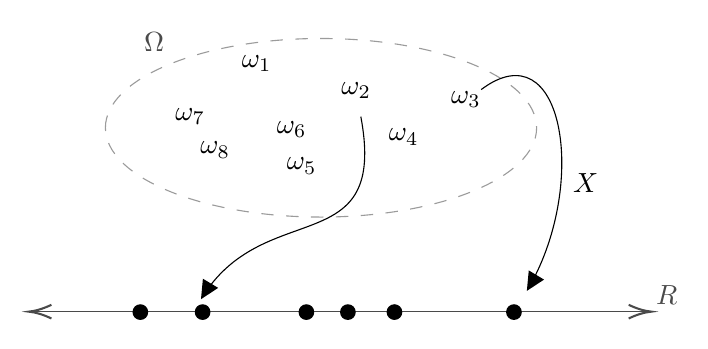
\begin{tikzpicture}[x=0.75pt,y=0.75pt,yscale=-1,xscale=1]
%uncomment if require: \path (0,300); %set diagram left start at 0, and has height of 300

%Shape: Ellipse [id:dp9108797218897698] 
\draw  [color={rgb, 255:red, 155; green, 155; blue, 155 }  ,draw opacity=1 ][dash pattern={on 4.5pt off 4.5pt}] (56.95,71.41) .. controls (56.95,47.65) and (103.46,28.39) .. (160.83,28.39) .. controls (218.21,28.39) and (264.71,47.65) .. (264.71,71.41) .. controls (264.71,95.17) and (218.21,114.43) .. (160.83,114.43) .. controls (103.46,114.43) and (56.95,95.17) .. (56.95,71.41) -- cycle ;
%Straight Lines [id:da6842961904360465] 
\draw [color={rgb, 255:red, 74; green, 74; blue, 74 }  ,draw opacity=1 ]   (22,160) -- (318,160) ;
\draw [shift={(320,160)}, rotate = 180] [color={rgb, 255:red, 74; green, 74; blue, 74 }  ,draw opacity=1 ][line width=0.75]    (10.93,-3.29) .. controls (6.95,-1.4) and (3.31,-0.3) .. (0,0) .. controls (3.31,0.3) and (6.95,1.4) .. (10.93,3.29)   ;
\draw [shift={(20,160)}, rotate = 0] [color={rgb, 255:red, 74; green, 74; blue, 74 }  ,draw opacity=1 ][line width=0.75]    (10.93,-3.29) .. controls (6.95,-1.4) and (3.31,-0.3) .. (0,0) .. controls (3.31,0.3) and (6.95,1.4) .. (10.93,3.29)   ;
%Shape: Circle [id:dp7950112027979597] 
\draw  [draw opacity=0][fill={rgb, 255:red, 0; green, 0; blue, 0 }  ,fill opacity=1 ] (100,160.21) .. controls (100,158.12) and (101.69,156.43) .. (103.79,156.43) .. controls (105.88,156.43) and (107.57,158.12) .. (107.57,160.21) .. controls (107.57,162.31) and (105.88,164) .. (103.79,164) .. controls (101.69,164) and (100,162.31) .. (100,160.21) -- cycle ;
%Shape: Circle [id:dp6131304198024731] 
\draw  [draw opacity=0][fill={rgb, 255:red, 0; green, 0; blue, 0 }  ,fill opacity=1 ] (170,160.21) .. controls (170,158.12) and (171.69,156.43) .. (173.79,156.43) .. controls (175.88,156.43) and (177.57,158.12) .. (177.57,160.21) .. controls (177.57,162.31) and (175.88,164) .. (173.79,164) .. controls (171.69,164) and (170,162.31) .. (170,160.21) -- cycle ;
%Shape: Circle [id:dp9238073836570526] 
\draw  [draw opacity=0][fill={rgb, 255:red, 0; green, 0; blue, 0 }  ,fill opacity=1 ] (192.43,160.21) .. controls (192.43,158.12) and (194.12,156.43) .. (196.21,156.43) .. controls (198.31,156.43) and (200,158.12) .. (200,160.21) .. controls (200,162.31) and (198.31,164) .. (196.21,164) .. controls (194.12,164) and (192.43,162.31) .. (192.43,160.21) -- cycle ;
%Shape: Circle [id:dp2974634348831592] 
\draw  [draw opacity=0][fill={rgb, 255:red, 0; green, 0; blue, 0 }  ,fill opacity=1 ] (250,160.21) .. controls (250,158.12) and (251.69,156.43) .. (253.79,156.43) .. controls (255.88,156.43) and (257.57,158.12) .. (257.57,160.21) .. controls (257.57,162.31) and (255.88,164) .. (253.79,164) .. controls (251.69,164) and (250,162.31) .. (250,160.21) -- cycle ;
%Shape: Circle [id:dp34244152371437553] 
\draw  [draw opacity=0][fill={rgb, 255:red, 0; green, 0; blue, 0 }  ,fill opacity=1 ] (70,160.21) .. controls (70,158.12) and (71.69,156.43) .. (73.79,156.43) .. controls (75.88,156.43) and (77.57,158.12) .. (77.57,160.21) .. controls (77.57,162.31) and (75.88,164) .. (73.79,164) .. controls (71.69,164) and (70,162.31) .. (70,160.21) -- cycle ;
%Shape: Circle [id:dp8457167113190215] 
\draw  [draw opacity=0][fill={rgb, 255:red, 0; green, 0; blue, 0 }  ,fill opacity=1 ] (150,160.21) .. controls (150,158.12) and (151.69,156.43) .. (153.79,156.43) .. controls (155.88,156.43) and (157.57,158.12) .. (157.57,160.21) .. controls (157.57,162.31) and (155.88,164) .. (153.79,164) .. controls (151.69,164) and (150,162.31) .. (150,160.21) -- cycle ;
%Curve Lines [id:da9264222857198537] 
\draw    (238,53) .. controls (277.4,23.45) and (289.77,97.58) .. (261.33,147.73) ;
\draw [shift={(260,150)}, rotate = 301.01] [fill={rgb, 255:red, 0; green, 0; blue, 0 }  ][line width=0.08]  [draw opacity=0] (8.93,-4.29) -- (0,0) -- (8.93,4.29) -- cycle    ;
%Curve Lines [id:da22175284361216296] 
\draw    (180,66) .. controls (193.09,135.65) and (134.93,104.82) .. (104.38,151.8) ;
\draw [shift={(103,154)}, rotate = 301.01] [fill={rgb, 255:red, 0; green, 0; blue, 0 }  ][line width=0.08]  [draw opacity=0] (8.93,-4.29) -- (0,0) -- (8.93,4.29) -- cycle    ;

% Text Node
\draw (89.43,60.87) node [anchor=north west][inner sep=0.75pt]    {$\omega _{7}$};
% Text Node
\draw (138.29,67.29) node [anchor=north west][inner sep=0.75pt]    {$\omega _{6}$};
% Text Node
\draw (101.43,77.01) node [anchor=north west][inner sep=0.75pt]    {$\omega _{8}$};
% Text Node
\draw (143.14,84.71) node [anchor=north west][inner sep=0.75pt]    {$\omega _{5}$};
% Text Node
\draw (169.43,48.4) node [anchor=north west][inner sep=0.75pt]    {$\omega _{2}$};
% Text Node
\draw (192.29,70.77) node [anchor=north west][inner sep=0.75pt]    {$\omega _{4}$};
% Text Node
\draw (121.43,35.38) node [anchor=north west][inner sep=0.75pt]    {$\omega _{1}$};
% Text Node
\draw (222.29,52.8) node [anchor=north west][inner sep=0.75pt]    {$\omega _{3}$};
% Text Node
\draw (74.29,24.28) node [anchor=north west][inner sep=0.75pt]  [color={rgb, 255:red, 74; green, 74; blue, 74 }  ,opacity=1 ]  {$\Omega $};
% Text Node
\draw (321,158) node [anchor=south west] [inner sep=0.75pt]  [color={rgb, 255:red, 74; green, 74; blue, 74 }  ,opacity=1 ]  {$\mathbb{R}$};
% Text Node
\draw (281,92) node [anchor=north west][inner sep=0.75pt]    {$X$};


\end{tikzpicture}

\end{center}

% \clearpage

\subsection{Probability Mass Functions}

With the introduction of discrete random variables, we can change our view from probabilities of events occurring to the probabilities that a discrete random variable takes on specific values. A nice way to do this is by introducing the \emph{probability mass function}.

\begin{definition}[Probability Mass Function]
	The \vocab{probability mass function} or \vocab{pmf} of a discrete random variable $X$ is a function $p_X: \R \rightarrow [0, 1]$ defined by
	$$
	p_X(x) = \PP(X = x) = \PP(\{ \omega \in \Omega : X(\omega) = x\}).
	$$
\end{definition}

It turns out that the probability mass function encodes pretty much all information about the discrete random variable $X$, so much so that if we have some function $p_X$ that acts like a probability mass function, we can say things like `let $X$ be a random variable taking value $x_i$ with probability $p_X(x_i)$' and have it be completely well defined.

\begin{theorem}
	Let $p_X : \R \rightarrow [0, 1]$ be a function such that $p_X(x) \neq 0$ for countably many $x$ and $\sum_{x \in \R} p_X(x) = 1$. Then there is a probability space $(\Omega, \FF, \PP)$ and a random variable $X$ on this space where $X$ has probability mass function $p_X$.
\end{theorem}
\begin{proof}
	Take $\Omega = \{x \in \R : p_X(x) \neq 0\}$, $\FF$ to be all subsets of $\Omega$, and 
	$$
	\PP(A) = \sum_{\omega \in A} p_X(\omega) \quad \text{for }A \in \FF,
	$$
	and define $X : \Omega \rightarrow \R$ by $X(\omega) = \omega$.
\end{proof}


\subsection{Expected Value}

A common question when dealing with discrete random variables is `what is the mean of this discrete random variable?'. Thinking back to our 
lecture hall example, this would correspond with asking what the mean test score in the lecture hall was.
We answer such questions by defining the \emph{expectation} of a random variable.

\begin{definition}[Expected Value]
	If $X$ is a discrete random variable, we define the \vocab{expected value} of $X$ to be
	$$
\EE[X] = \sum_{x \in \img X} x \PP(X = x)
	$$
	whenever this sum converges absolutely\footnote{We require this because we rearranging the sum shouldn't change the expected value -- see Analysis I.}.
\end{definition}

There are a few `tricks' which make the computation of expected value somewhat easier. For example, if we have a discrete random variable defined on some probability space $(\Omega, \FF, \PP)$, then we can sum over the elements of $\Omega$ rather than the elements of $\img X$.
Also, since random variables are really just functions, we can obtain new random variables by composing them with other functions, for example $X \mapsto X^2$. In such scenarios, we can use a seemingly obvious result.

\begin{theorem}[Law of The Subconscious Statistician]
	If $X$ is a discrete random variable and $g: \R \rightarrow \R$, then
	$$
\EE[g(X)] = \sum_{x \in \img X} g(x) \PP(X = x),
	$$
	whenever this sum converges absolutely.
\end{theorem}
\begin{proof}
	Let $Y = g(X)$ be a discrete random variable. Then
	\begin{align*}
		\EE[Y] &= \sum_{y \in \img Y} y \PP(Y = y) = \sum_{y \in \img Y} y \sum_{x \in \img X : g(x) = y} \PP(X = x)  \\
		&= \sum_{x \in \img X} g(x) \PP(X = x),
	\end{align*}
	provided this converges absolutely.
\end{proof}

Another thing we can do very easily is find the expected value of a sum of random variables, using \emph{linearity of expectation}.

\begin{theorem}[Linearity of Expectation]
	For any random variables $X_1, X_2, \dots, X_n$ for which the following expectations exist,
	$$
\EE\left[X_1 + \cdots + X_n\right]= \EE[X_1] + \cdots + \EE[X_n].
	$$
\end{theorem}
\begin{proof}
	We sum over the elements of the sample space $\Omega$ to get
	\begin{align*}
		\EE[X] &= \sum_{\omega \in \Omega} p(\omega)[X_1(\omega) + \cdots + X_n(\omega)]\\
		&= \sum_{\omega \in \Omega} p(\omega) X_1(\omega) + \cdots + \sum_{\omega \in \Omega} p(\omega) X_n(\omega)\\&= \EE[X_1] + \cdots + \EE[X_n].
	\end{align*}
\end{proof}

It's important to note that there's absolutely no requirement that the random variables be independent for this to hold -- one of the reasons why it's an incredibly useful result!

So if expected value measures something like the `mean' of a random variable, it's natural to think about how we can measure how we can expect the random variable deviates from this mean. This is done through the notion of \emph{variance}.

\begin{definition}[Variance]
	The \vocab{variance} $\var(X)$ of a discrete random variable $X$ is defined to be
	$$
\var(X) = \EE[(X - \EE[X])^2].
	$$
\end{definition}

By just working through the definitions we can see that $\var(X) = \EE[X^2] - \EE[X]^2$, which is often an easy way to calculate this quantity.

\subsection{Indicator Functions}

There's one type of random variable which is so useful that it needs to be brought to your attention immediately -- indicator functions.

\begin{definition}[Indicator Functions]
	The \vocab{indicator function} of an event $A$ is the random variable $\ii_A$ where
	$$
\ii_A(\omega) = \begin{cases}
	1 &\mbox{if } \omega  \in A, \\
	0 &\mbox{if } \omega  \not \in A.
   \end{cases}
	$$
\end{definition}

Indicator functions have nice algebraic facts which reflect common ways to manipulate events:
\begin{align*}
	\ii_{A^c} &= 1 - \ii_A, \\
	\ii_{A \cap B} &= \ii_A \ii_B, \\
	\ii_{A \cup B} &= \ii_A + \ii_B - \ii_A \ii_B.
\end{align*}
Still one of the best things about indicator functions is that they allow us to talk about probabilities of events using expectations, since
$$
\EE[\ii_A]= \PP(A).
$$
All of these properties are straightforward and easy to check (just do casework), but they can make proving things and solving problems much easier. Nontrivial example time!

\begin{example}[Solving Problems With Indicator Functions]
A total of $n$ bar magnets are placed end to end in a line with random independent orientations. Adjacent like poles repel, ends with opposite polarities join to form blocks. Let $X$ be the number of blocks of joined magnets. Find $\mathbb{E}[X]$ and $\var(X)$.
\end{example}
\begin{proof}[Solution]
	The situation looks something like this:
	\begin{center}
		

\tikzset{every picture/.style={line width=0.75pt}} %set default line width to 0.75pt        

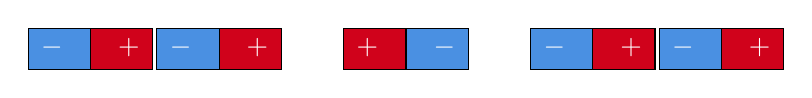
\begin{tikzpicture}[x=0.75pt,y=0.75pt,yscale=-1,xscale=1]
%uncomment if require: \path (0,300); %set diagram left start at 0, and has height of 300

%Shape: Rectangle [id:dp25601061256284363] 
\draw  [fill={rgb, 255:red, 74; green, 144; blue, 226 }  ,fill opacity=1 ] (78,230) -- (108,230) -- (108,250) -- (78,250) -- cycle ;
%Shape: Rectangle [id:dp6474954982899106] 
\draw  [fill={rgb, 255:red, 208; green, 2; blue, 27 }  ,fill opacity=1 ] (108,230) -- (138,230) -- (138,250) -- (108,250) -- cycle ;
%Shape: Rectangle [id:dp4965245878027762] 
\draw  [fill={rgb, 255:red, 74; green, 144; blue, 226 }  ,fill opacity=1 ] (140,230) -- (170,230) -- (170,250) -- (140,250) -- cycle ;
%Shape: Rectangle [id:dp1858582011582739] 
\draw  [fill={rgb, 255:red, 208; green, 2; blue, 27 }  ,fill opacity=1 ] (170,230) -- (200,230) -- (200,250) -- (170,250) -- cycle ;
%Shape: Rectangle [id:dp8867339379180033] 
\draw  [fill={rgb, 255:red, 208; green, 2; blue, 27 }  ,fill opacity=1 ] (230,230) -- (260,230) -- (260,250) -- (230,250) -- cycle ;
%Shape: Rectangle [id:dp33998768810132374] 
\draw  [fill={rgb, 255:red, 74; green, 144; blue, 226 }  ,fill opacity=1 ] (260,230) -- (290,230) -- (290,250) -- (260,250) -- cycle ;
%Shape: Rectangle [id:dp09533432318082213] 
\draw  [fill={rgb, 255:red, 74; green, 144; blue, 226 }  ,fill opacity=1 ] (320,230) -- (350,230) -- (350,250) -- (320,250) -- cycle ;
%Shape: Rectangle [id:dp9775009294983759] 
\draw  [fill={rgb, 255:red, 208; green, 2; blue, 27 }  ,fill opacity=1 ] (350,230) -- (380,230) -- (380,250) -- (350,250) -- cycle ;
%Shape: Rectangle [id:dp24270866646840328] 
\draw  [fill={rgb, 255:red, 74; green, 144; blue, 226 }  ,fill opacity=1 ] (382,230) -- (412,230) -- (412,250) -- (382,250) -- cycle ;
%Shape: Rectangle [id:dp11919818567548779] 
\draw  [fill={rgb, 255:red, 208; green, 2; blue, 27 }  ,fill opacity=1 ] (412,230) -- (442,230) -- (442,250) -- (412,250) -- cycle ;

% Text Node
\draw (120,233.4) node [anchor=north west][inner sep=0.75pt]  [color={rgb, 255:red, 255; green, 255; blue, 255 }  ,opacity=1 ]  {$+$};
% Text Node
\draw (83,233.4) node [anchor=north west][inner sep=0.75pt]  [color={rgb, 255:red, 255; green, 255; blue, 255 }  ,opacity=1 ]  {$-$};
% Text Node
\draw (182,233.4) node [anchor=north west][inner sep=0.75pt]  [color={rgb, 255:red, 255; green, 255; blue, 255 }  ,opacity=1 ]  {$+$};
% Text Node
\draw (145,233.4) node [anchor=north west][inner sep=0.75pt]  [color={rgb, 255:red, 255; green, 255; blue, 255 }  ,opacity=1 ]  {$-$};
% Text Node
\draw (272,233.4) node [anchor=north west][inner sep=0.75pt]  [color={rgb, 255:red, 255; green, 255; blue, 255 }  ,opacity=1 ]  {$-$};
% Text Node
\draw (235,233.4) node [anchor=north west][inner sep=0.75pt]  [color={rgb, 255:red, 255; green, 255; blue, 255 }  ,opacity=1 ]  {$+$};
% Text Node
\draw (362,233.4) node [anchor=north west][inner sep=0.75pt]  [color={rgb, 255:red, 255; green, 255; blue, 255 }  ,opacity=1 ]  {$+$};
% Text Node
\draw (325,233.4) node [anchor=north west][inner sep=0.75pt]  [color={rgb, 255:red, 255; green, 255; blue, 255 }  ,opacity=1 ]  {$-$};
% Text Node
\draw (424,233.4) node [anchor=north west][inner sep=0.75pt]  [color={rgb, 255:red, 255; green, 255; blue, 255 }  ,opacity=1 ]  {$+$};
% Text Node
\draw (387,233.4) node [anchor=north west][inner sep=0.75pt]  [color={rgb, 255:red, 255; green, 255; blue, 255 }  ,opacity=1 ]  {$-$};


\end{tikzpicture}

	\end{center}
	Let $\ii_i$ be the indicator function for magnets $i$ and $i+1$ repelling, for $1 \leq i \leq n - 1$. We can then rewrite $X$ as 
	$$
	X = \ii_1 + \ii_2 + \cdots + \ii_{n - 1} + 1.
	$$
	Then since $\EE[\ii_i] = \PP(\text{two magnets of random orientation repel}) = 1/2$, we have
	\begin{align*}
		\EE[X] &= \EE[\ii_1] + \cdots + \EE[\ii_{n - 1}] + 1\\
		&= \frac{1}{2} + \cdots + \frac{1}{2} + 1 = \frac{n + 1}{2}.
	\end{align*}
	To compute the variance, we need to calculate $\EE[X^2]$. Writing $S = \ii_1 + \cdots + \ii_{n-1}$, so that $X = 1 + S$, we can expand
	$$
	X^2 = 1 + 2S + S^2 = 1 + 2S + (\ii_1^2 + \cdots + \ii_{n-1}^2) + \sum_{i \neq j} \ii_i \ii_j = 1 + 3S + \sum_{i \neq j} \ii_i \ii_j,
	$$
	using that $\ii_i^2 = \ii_i$ for indicators. Now $\EE[\ii_i \ii_j] = \PP(\text{both pairs repel}) = 1/4$ for $i \neq j$ (the two events involve at least one distinct magnet orientation each, and one can check they are independent), and there are $(n-1)(n-2)$ ordered pairs $i \neq j$. So
	\begin{align*}
		\EE[X^2] &= 1 + 3 \cdot \frac{n - 1}{2} + (n - 1)(n - 2)\cdot\frac{1}{4} = \frac{3n - 1}{2} + \frac{(n-1)(n-2)}{4},
	\end{align*}
	and thus
	\begin{align*}
		\var(X) &= \EE[X^2] - \EE[X]^2 = \frac{3n - 1}{2} + \frac{(n-1)(n-2)}{4} - \frac{(n + 1)^2}{4} \\
		&= \frac{2(3n - 1) + (n^2 - 3n + 2) - (n^2 + 2n + 1)}{4} = \frac{n - 1}{4}.
	\end{align*}
	As a sanity check: the indicators $\ii_1, \dots, \ii_{n-1}$ are actually mutually independent (each depends on whether consecutive orientations differ), so $X - 1$ is a sum of $n - 1$ independent `coin flips' and we should expect variance $(n-1) \cdot \frac{1}{2} \cdot \frac{1}{2} = \frac{n-1}{4}$, which matches.
\end{proof}

One more nice trick with indicators: if $X$ is a random variable taking values in the non-negative integers, then writing $X = \sum_{k \geq 1} \ii_{\{X \geq k\}}$ (an integer $m$ is the sum of $m$ ones!) and taking expectations gives the occasionally very convenient formula
$$
\EE[X] = \sum_{k = 1}^{\infty} \PP(X \geq k).
$$

\subsection{A Zoo of Standard Distributions}

There are a handful of distributions that show up over and over again, both in applications and throughout the rest of this course, so we will now go through them and compute their expectations and variances. Recall that the distribution of a discrete random variable is specified entirely by its probability mass function.

\subsubsection*{The Bernoulli Distribution}

The simplest random experiment imaginable has two outcomes: success (with probability $p$) or failure. We say $X$ has the \vocab{Bernoulli distribution} with parameter $p \in [0, 1]$, written $X \sim \mathrm{Bernoulli}(p)$, if
$$
\PP(X = 1) = p, \qquad \PP(X = 0) = 1 - p.
$$
Immediately we get $\EE[X] = p$, and since $X^2 = X$,
$$
\var(X) = \EE[X^2] - \EE[X]^2 = p - p^2 = p(1-p).
$$
Of course, an indicator function $\ii_A$ is exactly a Bernoulli random variable with parameter $\PP(A)$.

\subsubsection*{The Binomial Distribution}

Now toss the same coin $n$ times independently, and count the number of successes. This gives the \vocab{binomial distribution} $X \sim \mathrm{Bin}(n, p)$, with
$$
\PP(X = k) = \binom{n}{k} p^k (1 - p)^{n - k}, \quad k \in \{0, 1, \dots, n\},
$$
the binomial coefficient counting which of the $n$ trials were the successes. The binomial theorem shows these probabilities sum to $1$ (hence the name).

Writing $X = \ii_1 + \cdots + \ii_n$ as a sum of indicators of success in each trial, linearity of expectation instantly gives
$$
\EE[X] = np.
$$
For the variance, the slickest elementary route is via $\EE[X(X-1)]$ (a \emph{factorial moment} -- these interact very well with binomial coefficients):
\begin{align*}
	\EE[X(X - 1)] &= \sum_{k = 2}^{n} k(k-1)\binom{n}{k}p^k (1-p)^{n - k} \\
	&= n(n-1)p^2 \sum_{k = 2}^{n} \binom{n - 2}{k - 2} p^{k - 2}(1 - p)^{n - k} = n(n - 1)p^2,
\end{align*}
using the identity $k(k-1)\binom{n}{k} = n(n-1)\binom{n-2}{k-2}$ and then the binomial theorem. Hence
$$
\var(X) = \EE[X(X-1)] + \EE[X] - \EE[X]^2 = n(n-1)p^2 + np - n^2p^2 = np(1 - p).
$$

\begin{remark}[The Multinomial Distribution]
	If each trial has not two but $k$ possible outcomes, with probabilities $p_1, \dots, p_k$ summing to $1$, then the vector $(N_1, \dots, N_k)$ of counts of each outcome over $n$ independent trials has the \vocab{multinomial distribution}:
	$$
	\PP(N_1 = n_1, \dots, N_k = n_k) = \binom{n}{n_1, \dots, n_k}p_1^{n_1}\cdots p_k^{n_k},
	$$
	for $n_1 + \cdots + n_k = n$, with the multinomial coefficient counting the arrangements of outcomes among the trials. Each marginal $N_i$ is $\mathrm{Bin}(n, p_i)$.
\end{remark}

\subsubsection*{The Geometric Distribution}

Instead of a fixed number of tosses, toss the coin repeatedly until the first success, and let $X$ be the number of tosses used. This is the \vocab{geometric distribution} $X \sim \mathrm{Geom}(p)$ (with $p > 0$), where
$$
\PP(X = k) = (1 - p)^{k - 1} p, \quad k \in \{1, 2, 3, \dots \},
$$
since we need $k - 1$ failures followed by a success\footnote{Some authors instead count the number of \emph{failures} before the first success, giving pmf $(1-p)^k p$ on $\{0, 1, 2, \dots\}$ -- watch out for the convention in use.}. Summing a geometric series confirms the total probability is $1$ -- in particular, the first success comes eventually with probability $1$.

For the expectation, note $\PP(X \geq k) = (1-p)^{k - 1}$ (the first $k - 1$ tosses all fail), so using our tail-sum formula,
$$
\EE[X] = \sum_{k = 1}^{\infty} \PP(X \geq k) = \sum_{k = 1}^{\infty} (1 - p)^{k - 1} = \frac{1}{p},
$$
which matches intuition: an event of probability $p$ takes about $1/p$ attempts to see. For the variance we again use factorial moments, this time with the second derivative of the geometric series $\sum_{k} q^k = (1-q)^{-1}$:
$$
\EE[X(X-1)] = \sum_{k = 2}^{\infty} k(k - 1)(1-p)^{k-1} p = p(1-p)\sum_{k=2}^{\infty} k(k-1)(1-p)^{k - 2} = \frac{2(1-p)}{p^2},
$$
and thus
$$
\var(X) = \frac{2(1-p)}{p^2} + \frac{1}{p} - \frac{1}{p^2} = \frac{1 - p}{p^2}.
$$

The geometric distribution has a property worth flagging now, as we will meet its continuous cousin later: it is \emph{memoryless}. If the first $s$ tosses were all failures, the number of \emph{further} tosses needed is distributed just like a fresh geometric:
$$
\PP(X > s + t \mid X > s) = \frac{(1-p)^{s + t}}{(1 - p)^s} = (1-p)^t = \PP(X > t).
$$
The coin does not remember its past -- which is also why the `gambler's fallacy' (a run of losses making a win `due') is a fallacy.

\subsubsection*{The Hypergeometric Distribution}

Suppose an urn contains $N$ balls, $K$ of which are red, and we draw $n$ balls \emph{without replacement}. The number $X$ of red balls drawn has the \vocab{hypergeometric distribution}, with
$$
\PP(X = k) = \frac{\binom{K}{k}\binom{N - K}{n - k}}{\binom{N}{n}},
$$
for the possible values of $k$. Indicators make the expectation painless: letting $\ii_i$ indicate that the $i$-th draw is red, each draw is (by symmetry) equally likely to be any of the $N$ balls, so $\EE[\ii_i] = K/N$ and
$$
\EE[X] = \frac{nK}{N}.
$$
Note this matches the binomial mean with $p = K/N$ -- drawing without replacement doesn't change the expectation, though it does shrink the variance.

\subsubsection*{The Poisson Distribution}

Our final distribution models the number of events occurring in a fixed window of time, when events occur `at a constant rate, independently': the number of buses passing in an hour, misprints on a page, radioactive decays in a second, and so on. We say $X$ has the \vocab{Poisson distribution} with parameter $\lambda > 0$, written $X \sim \mathrm{Poisson}(\lambda)$, if
$$
\PP(X = k) = e^{-\lambda}\frac{\lambda^k}{k!}, \quad k \in \{0, 1, 2, \dots\}.
$$
The total probability is $e^{-\lambda}\sum_k \lambda^k / k! = e^{-\lambda}e^{\lambda} = 1$, as needed. The expectation is
$$
\EE[X] = \sum_{k = 1}^{\infty} k e^{-\lambda} \frac{\lambda^k}{k!} = \lambda e^{-\lambda} \sum_{k = 1}^{\infty} \frac{\lambda^{k - 1}}{(k-1)!} = \lambda,
$$
so the parameter $\lambda$ is exactly the average number of events. Similarly $\EE[X(X-1)] = \lambda^2 e^{-\lambda}\sum_{k \geq 2} \lambda^{k-2}/(k-2)! = \lambda^2$, giving
$$
\var(X) = \lambda^2 + \lambda - \lambda^2 = \lambda.
$$
The mean and the variance are both $\lambda$ -- a distinctive fingerprint of the Poisson distribution.

Where does the Poisson distribution come from? It arises naturally as a limit of binomials with many trials, each individually unlikely -- this is sometimes called the \emph{law of rare events}.

\begin{theorem}[Poisson Approximation to the Binomial]
	Fix $\lambda > 0$, and let $X_n \sim \mathrm{Bin}(n, \lambda/n)$. Then for each fixed $k \geq 0$,
	$$
	\PP(X_n = k) \longrightarrow e^{-\lambda} \frac{\lambda^k}{k!} \quad \text{as } n \rightarrow \infty.
	$$
\end{theorem}
\begin{proof}
	We compute directly:
	\begin{align*}
		\PP(X_n = k) &= \binom{n}{k}\left(\frac{\lambda}{n}\right)^k \left(1 - \frac{\lambda}{n}\right)^{n - k} \\
		&= \frac{\lambda^k}{k!} \cdot \frac{n(n-1)\cdots(n - k + 1)}{n^k} \cdot \left(1 - \frac{\lambda}{n}\right)^{n} \left(1 - \frac{\lambda}{n}\right)^{-k}.
	\end{align*}
	As $n \rightarrow \infty$ with $k$ fixed, the middle factor tends to $1$, the last factor tends to $1$, and $(1 - \lambda/n)^n \rightarrow e^{-\lambda}$. So $\PP(X_n = k) \rightarrow e^{-\lambda}\lambda^k/k!$ as claimed.
\end{proof}

To interpret this: divide an hour into $n$ tiny intervals, and suppose a bus arrives in each interval with probability $\lambda/n$, independently. The number of buses in the hour is $\mathrm{Bin}(n, \lambda/n)$, and letting the intervals shrink gives exactly $\mathrm{Poisson}(\lambda)$.


\section{Multiple Random Variables}

Most interesting probabilistic questions involve the interaction of \emph{several} random variables -- and this is where notions like independence, covariance and conditional expectation come into play.

\subsection{Joint Distributions and Independence}

So far we have studied random variables one at a time. To capture how several random variables interact, we record all of their values at once.

\begin{definition}[Joint Distribution]
	Let $X_1, \dots, X_n$ be discrete random variables on a probability space. Their \vocab{joint distribution} is the collection of probabilities
	$$
	\PP(X_1 = x_1, X_2 = x_2, \dots, X_n = x_n),
	$$
	over all possible values $x_1, \dots, x_n$.
\end{definition}

The joint distribution knows everything about the individual random variables: summing out all but one variable recovers what is called the \vocab{marginal distribution},
$$
\PP(X_1 = x_1) = \sum_{x_2, \dots, x_n} \PP(X_1 = x_1, X_2 = x_2, \dots, X_n = x_n),
$$
which is just the partition theorem in disguise. The converse fails badly -- the marginals alone don't determine the joint distribution, as they say nothing about how the variables \emph{depend} on each other. The simplest possible dependence structure is no dependence at all.

\begin{definition}[Independent Random Variables]
	Discrete random variables $X_1, \dots, X_n$ are \vocab{independent} if for all values $x_1, \dots, x_n$,
	$$
	\PP(X_1 = x_1, \dots, X_n = x_n) = \PP(X_1 = x_1) \cdots \PP(X_n = x_n).
	$$
\end{definition}

\begin{example}[Coin Tossing, Formally]
	Let's model tossing a biased coin $n$ times, formally. Take $\Omega = \{0, 1\}^n$, and for $\omega = (\omega_1, \dots, \omega_n)$ set
	$$
	\PP(\{\omega\}) = \prod_{k=1}^n p^{\omega_k}(1 - p)^{1 - \omega_k},
	$$
	and let $X_k(\omega) = \omega_k$ be the result of the $k$th toss. Then each $X_k \sim \mathrm{Bernoulli}(p)$, and multiplying out shows that $\PP(X_1 = x_1, \dots, X_n = x_n) = \prod_k \PP(X_k = x_k)$, so the tosses are genuinely independent in our formal sense. The number of heads $S_n = X_1 + \cdots + X_n$ then has the $\mathrm{Bin}(n, p)$ distribution.
\end{example}

A very useful consequence of independence is that expectations of products factorise.

\begin{theorem}[Expectation of a Product]
	If $X$ and $Y$ are independent discrete random variables and $f, g: \R \rightarrow \R$, then
	$$
	\EE[f(X)g(Y)] = \EE[f(X)] \, \EE[g(Y)],
	$$
	whenever the expectations on the right exist.
\end{theorem}
\begin{proof}
	Summing over the possible pairs of values,
	\begin{align*}
		\EE[f(X)g(Y)] &= \sum_{x, y} f(x)g(y)\PP(X = x, Y = y) \\
		&= \sum_{x, y} f(x)g(y)\PP(X = x)\PP(Y = y) \\
		&= \left(\sum_x f(x)\PP(X = x)\right)\left(\sum_y g(y) \PP(Y = y)\right) = \EE[f(X)]\,\EE[g(Y)],
	\end{align*}
	where the rearrangement is justified by absolute convergence.
\end{proof}

Contrast this with linearity of expectation, which required no independence whatsoever: for products, independence is really doing work.

We can also ask about the distribution of a \emph{sum} of independent random variables. Conditioning on the value of one of them gives
$$
\PP(X + Y = z) = \sum_y \PP(X = z - y, Y = y) = \sum_{y} \PP(X = z - y)\PP(Y = y),
$$
a formula known as the \vocab{convolution} of the two distributions.

\begin{example}[Sum of Independent Poissons]
	Let $X \sim \mathrm{Poisson}(\lambda)$ and $Y \sim \mathrm{Poisson}(\mu)$ be independent. Then
	\begin{align*}
		\PP(X + Y = n) &= \sum_{r = 0}^{n} e^{-\lambda}\frac{\lambda^r}{r!} \cdot e^{-\mu}\frac{\mu^{n - r}}{(n-r)!} \\
		&= \frac{e^{-(\lambda + \mu)}}{n!} \sum_{r = 0}^{n} \binom{n}{r}\lambda^r \mu^{n - r} = e^{-(\lambda + \mu)}\frac{(\lambda + \mu)^n}{n!},
	\end{align*}
	using the binomial theorem. So $X + Y \sim \mathrm{Poisson}(\lambda + \mu)$ -- the Poisson family is closed under adding independent members, which is exactly what you'd hope for from a distribution modelling counts of events (two independent streams of buses form one stream with the combined rate).
\end{example}

\subsection{Covariance}

If independence is the absence of dependence, we'd also like a way to \emph{measure} dependence. The first-order tool for this is covariance.

\begin{definition}[Covariance]
	The \vocab{covariance} of random variables $X$ and $Y$ is
	$$
	\cov(X, Y) = \EE[(X - \EE[X])(Y - \EE[Y])],
	$$
	whenever this exists.
\end{definition}

Roughly, $\cov(X, Y) > 0$ means $X$ and $Y$ tend to be large together, and $\cov(X, Y) < 0$ means one tends to be large when the other is small. Covariance has a pile of easily-verified properties, which we collect here.

\begin{proposition}[Properties of Covariance]
	For random variables $X, Y, Z$ and a constant $c$:
	\begin{enumerate}[label=(\roman*)]
		\item $\cov(X, Y) = \cov(Y, X)$, and $\cov(X, X) = \var(X)$,
		\item $\cov(X, Y) = \EE[XY] - \EE[X]\EE[Y]$,
		\item $\cov(cX, Y) = c\cov(X, Y)$ and $\cov(X + c, Y) = \cov(X, Y)$,
		\item $\cov(X + Y, Z) = \cov(X, Z) + \cov(Y, Z)$,
		\item $\var(X + Y) = \var(X) + \var(Y) + 2\cov(X, Y)$.
	\end{enumerate}
\end{proposition}
\begin{proof}
	Part (i) is immediate from the definition. For (ii), expand
	$$
	(X - \EE X)(Y - \EE Y) = XY - X \EE[Y] - Y \EE[X] + \EE[X]\EE[Y]
	$$
	and take expectations. Parts (iii) and (iv) then follow from linearity of expectation applied to (ii). For (v), write $\tilde{X} = X - \EE[X]$ and $\tilde{Y} = Y - \EE[Y]$; then
	$$
	\var(X + Y) = \EE[(\tilde X + \tilde Y)^2] = \EE[\tilde X^2] + \EE[\tilde Y^2] + 2\EE[\tilde X \tilde Y],
	$$
	which is exactly the claim.
\end{proof}

Iterating (iv) and (v) gives the general and very useful formula
$$
\var\left(\sum_{i = 1}^{n} X_i\right) = \sum_{i = 1}^{n} \var(X_i) + \sum_{i \neq j} \cov(X_i, X_j).
$$

If $X$ and $Y$ are independent, then $\EE[XY] = \EE[X]\EE[Y]$ by the product theorem, so property (ii) gives $\cov(X, Y) = 0$, and hence variance becomes additive:
$$
\var(X + Y) = \var(X) + \var(Y) \quad \text{for independent } X, Y.
$$
(This gives another derivation of the binomial variance $np(1-p)$, summing the variances of $n$ independent Bernoulli trials.)

It's very important to remember that the converse is \emph{false}: zero covariance does not imply independence.

\begin{example}[Uncorrelated but Dependent]
	Let $X_1, X_2, X_3$ be independent $\mathrm{Bernoulli}(1/2)$ random variables, and set $Y_i = 2X_i - 1$ (so the $Y_i$ are random signs), and consider $Z_1 = X_3 Y_1$ and $Z_2 = X_3 Y_2$. Then $\EE[Z_1] = \EE[Z_2] = 0$ and
	$$
	\cov(Z_1, Z_2) = \EE[Z_1 Z_2] = \EE[X_3^2]\,\EE[Y_1]\,\EE[Y_2] = 0,
	$$
	using independence of $X_3, Y_1, Y_2$. But $Z_1, Z_2$ are certainly not independent: since $Y_1, Y_2$ are never zero, $Z_1 = 0$ happens exactly when $X_3 = 0$, and likewise for $Z_2$, so
	$$
	\PP(Z_1 = 0, Z_2 = 0) = \PP(X_3 = 0) = \frac{1}{2} \neq \frac{1}{4} = \PP(Z_1 = 0)\PP(Z_2 = 0).
	$$
\end{example}

Since covariance scales with the variables (property (iii)), it is often more meaningful to normalise it, defining the \vocab{correlation}
$$
\corr(X, Y) = \frac{\cov(X, Y)}{\sqrt{\var(X)\var(Y)}},
$$
when the variances are finite and nonzero. We will see later (from the Cauchy-Schwarz inequality) that correlation always lies in $[-1, 1]$.

\subsection{Conditional Expectation}

We now bring conditioning into the world of random variables. If $B$ is an event with $\PP(B) > 0$, we define the \vocab{conditional expectation} of $X$ given $B$ to be
$$
\EE[X \mid B] = \frac{\EE[X \ii_B]}{\PP(B)} = \sum_x x \PP(X = x \mid B),
$$
the average of $X$ over only those outcomes lying in $B$. Just as knowing conditional probabilities in every scenario gives the total probability, conditional expectations recombine to give the full expectation.

\begin{theorem}[Law of Total Expectation]
	Let $\{B_1, B_2, \dots\}$ be disjoint events with $\bigcup_i B_i = \Omega$ and $\PP(B_i) > 0$. Then for any random variable $X$ for which $\EE[X]$ exists,
	$$
	\EE[X] = \sum_i \EE[X \mid B_i] \, \PP(B_i).
	$$
\end{theorem}
\begin{proof}
	Since $\ii_{B_1} + \ii_{B_2} + \cdots = 1$, we can write $X = \sum_i X\ii_{B_i}$, and taking expectations (using linearity, or countable additivity of expectation in the infinite case, applied first to non-negative parts) gives
	$$
	\EE[X] = \sum_i \EE[X \ii_{B_i}] = \sum_i \EE[X \mid B_i]\PP(B_i). \qedhere
	$$
\end{proof}

Now for a genuinely important idea. Given two random variables $X$ and $Y$, for each possible value $y$ of $Y$ we can compute the number $g(y) = \EE[X \mid Y = y]$. This defines a function of $y$, and plugging the random variable $Y$ back into it yields a \emph{random variable}
$$
\EE[X \mid Y] = g(Y),
$$
called the \vocab{conditional expectation of $X$ given $Y$}. You should think of $\EE[X \mid Y]$ as the best guess of $X$ made by someone who knows the value of $Y$: it is random precisely because $Y$ is.

\begin{example}
	Toss a biased coin $n$ times, let $X_i$ be the indicator that toss $i$ is a head, and let $Y_n = X_1 + \cdots + X_n$ be the total number of heads. What is $\EE[X_1 \mid Y_n]$?

	We compute, for $y \geq 1$,
	\begin{align*}
		\EE[X_1 \mid Y_n = y] = \PP(X_1 = 1 \mid Y_n = y) &= \frac{\PP(X_1 = 1, \, X_2 + \cdots + X_n = y - 1)}{\PP(Y_n = y)} \\
		&= \frac{p\binom{n - 1}{y - 1}p^{y-1}(1-p)^{n - y}}{\binom{n}{y}p^y(1-p)^{n-y}} = \frac{\binom{n-1}{y-1}}{\binom{n}{y}} = \frac{y}{n},
	\end{align*}
	and this also holds (trivially) for $y = 0$. So $\EE[X_1 \mid Y_n] = Y_n / n$. Note the answer doesn't even depend on $p$: given the total number of heads, each toss is equally likely to have contributed, by symmetry.
\end{example}

The key properties of conditional expectation are as follows.

\begin{proposition}[Properties of Conditional Expectation]
	Let $X, Y, Z$ be discrete random variables, and $c \in \R$. Then, whenever the relevant expectations exist:
	\begin{enumerate}[label=(\roman*)]
		\item (Linearity) $\EE[cX + Z \mid Y] = c\EE[X \mid Y] + \EE[Z \mid Y]$.
		\item (Tower property) $\EE\big[\EE[X \mid Y]\big] = \EE[X]$.
		\item (Taking out what is known) $\EE[h(Y) X \mid Y] = h(Y) \EE[X \mid Y]$ for any function $h$.
		\item (Independence) If $X$ and $Y$ are independent, then $\EE[X \mid Y] = \EE[X]$.
	\end{enumerate}
\end{proposition}
\begin{proof}
	Part (i) holds since $\EE[\,\cdot \mid Y = y]$ is an expectation with respect to the probability measure $\PP(\,\cdot \mid Y = y)$, and expectations are linear.

	For (ii), we use the law of total expectation with the partition $\{Y = y\}$:
	$$
	\EE\big[\EE[X \mid Y]\big] = \sum_y \EE[X \mid Y = y] \, \PP(Y = y) = \EE[X].
	$$
	For (iii), conditionally on $Y = y$ the random variable $h(Y)$ is just the constant $h(y)$, so
	$$
	\EE[h(Y)X \mid Y = y] = h(y)\EE[X \mid Y = y],
	$$
	and substituting $Y$ for $y$ gives the claim. Finally for (iv), if $X, Y$ are independent then $\PP(X = x \mid Y = y) = \PP(X = x)$ for every $y$, so $\EE[X \mid Y = y] = \EE[X]$ for all $y$.
\end{proof}

The tower property is used \emph{constantly} -- it lets us compute a difficult expectation by first conditioning on some helpful piece of information. We will lean on it heavily when we study branching processes.


\section{Inequalities and the Law of Large Numbers}

Exact computations are all well and good, but much of the power of probability theory comes from \emph{inequalities} -- results that let us bound probabilities and expectations with only partial information about a distribution. We will build up the standard toolkit, and then use it to prove our first genuine limit theorem.

Everything in this section works for arbitrary random variables (discrete or otherwise); the proofs we give need nothing beyond basic properties of expectation.

\subsection{Markov and Chebyshev}

Our first inequality says: a non-negative random variable with a small mean is unlikely to be large. Crude, but astonishingly useful.

\begin{theorem}[Markov's Inequality]
	Let $X \geq 0$ be a random variable. Then for any $a > 0$,
	$$
	\PP(X \geq a) \leq \frac{\EE[X]}{a}.
	$$
\end{theorem}
\begin{proof}
	The whole proof is the pointwise inequality $X \geq a \ii_{\{X \geq a\}}$, which is easily checked in both the cases $X \geq a$ and $X < a$ (using $X \geq 0$ for the latter). Taking expectations,
	$$
	\EE[X] \geq a \, \EE[\ii_{\{X \geq a\}}] = a\,\PP(X \geq a),
	$$
	and dividing by $a$ gives the result.
\end{proof}

Applying Markov's inequality to the squared deviation of $X$ from its mean gives a bound in terms of the variance -- a much sharper tool, since it captures fluctuations rather than just size.

\begin{theorem}[Chebyshev's Inequality]
	Let $X$ be a random variable with finite mean. Then for any $a > 0$,
	$$
	\PP\big(|X - \EE[X]| \geq a\big) \leq \frac{\var(X)}{a^2}.
	$$
\end{theorem}
\begin{proof}
	The event $\{|X - \EE[X]| \geq a\}$ is the same as the event $\{(X - \EE[X])^2 \geq a^2\}$, and applying Markov's inequality to the non-negative random variable $(X - \EE[X])^2$ gives
	$$
	\PP\big((X - \EE[X])^2 \geq a^2\big) \leq \frac{\EE[(X - \EE[X])^2]}{a^2} = \frac{\var(X)}{a^2}. \qedhere
	$$
\end{proof}

In words: a random variable is unlikely to be many standard deviations away from its mean -- the probability of being at least $k$ standard deviations away is at most $1/k^2$, whatever the distribution. This universality is what makes Chebyshev so valuable.

\subsection{Cauchy-Schwarz}

The next inequality should look familiar from any setting with an inner product; expectation of a product behaves exactly like one.

\begin{theorem}[Cauchy-Schwarz Inequality]
	For random variables $X$ and $Y$,
	$$
	\left|\EE[XY]\right| \leq \sqrt{\EE[X^2]\,\EE[Y^2]}.
	$$
\end{theorem}
\begin{proof}
	If either of $\EE[X^2]$ or $\EE[Y^2]$ is infinite the inequality is trivial, so assume both are finite (note $|XY| \leq \frac{1}{2}(X^2 + Y^2)$ ensures $\EE[XY]$ exists). Further, if $\EE[Y^2] = 0$ then $Y = 0$ with probability $1$ and both sides vanish, so assume $\EE[Y^2] > 0$.

	Now for any $t \in \R$, we have $(X - tY)^2 \geq 0$, so taking expectations,
	$$
	f(t) = \EE[(X - tY)^2] = \EE[X^2] - 2t\,\EE[XY] + t^2\,\EE[Y^2] \geq 0.
	$$
	This is a quadratic in $t$ which never goes negative, so evaluating at its minimum $t^* = \EE[XY]/\EE[Y^2]$,
	$$
	0 \leq f(t^*) = \EE[X^2] - \frac{\EE[XY]^2}{\EE[Y^2]},
	$$
	which rearranges to $\EE[XY]^2 \leq \EE[X^2]\EE[Y^2]$, as required.
\end{proof}

\begin{remark}
	Chasing through the proof shows when equality holds: we need $\EE[(X - t^* Y)^2] = 0$, which forces $X = t^* Y$ with probability $1$. So equality in Cauchy-Schwarz means the variables are (almost surely) proportional.
\end{remark}

Applying Cauchy-Schwarz to the centred variables $X - \EE[X]$ and $Y - \EE[Y]$ gives
$$
|\cov(X, Y)| \leq \sqrt{\var(X)\var(Y)},
$$
which is exactly the promised fact that correlations lie in $[-1, 1]$, with $\pm 1$ attained precisely for (almost surely) linear relationships.

\subsection{Jensen's Inequality}

Our final inequality concerns \emph{convex} functions. Recall that $f: \R \rightarrow \R$ is \vocab{convex} if for all $x, y \in \R$ and $t \in [0, 1]$,
$$
f(tx + (1 - t)y) \leq tf(x) + (1 - t)f(y),
$$
that is, chords of the graph of $f$ lie above the graph. We say $f$ is \vocab{concave} if $-f$ is convex.

\begin{center}
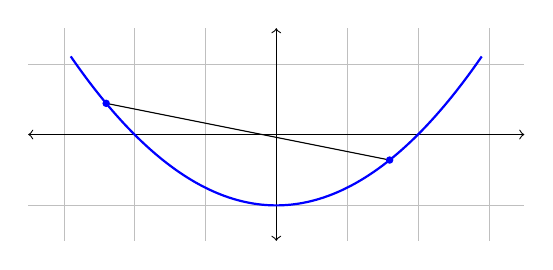
\begin{tikzpicture}[scale=0.9]
	\draw[ultra thin, color=lightgray] (-3.5,-1.5) grid (3.5,1.5);
	\draw[<->] (-3.5,0) -- (3.5,0);
	\draw[<->] (0,-1.5) -- (0,1.5);
	\draw[thick, samples=100, smooth, domain=-2.9:2.9, color=blue] plot (\x, {\x*\x/4 - 1});
	\draw (-2.4,0.44) -- (1.6,-0.36);
	\fill[blue] (-2.4,0.44) circle (1.5pt);
	\fill[blue] (1.6,-0.36) circle (1.5pt);
\end{tikzpicture}
\end{center}

The definition of convexity says that $f$ of an average of \emph{two} points is at most the average of the values. Jensen's inequality upgrades this from two-point averages to arbitrary expectations.

\begin{theorem}[Jensen's Inequality]
	Let $X$ be a random variable with finite mean and let $f: \R \rightarrow \R$ be convex. Then
	$$
	\EE[f(X)] \geq f(\EE[X]).
	$$
\end{theorem}

A helpful mnemonic for the direction: $f(x) = x^2$ is convex, and $\EE[X^2] \geq \EE[X]^2$ is just the statement $\var(X) \geq 0$.

The proof rests on a fundamental geometric property of convex functions: at every point, there is a line through the graph lying entirely below it (a \emph{supporting line}).

\begin{lemma}[Supporting Lines]
	Let $f$ be convex and $m \in \R$. Then there exist $a, b \in \R$ such that $f(m) = am + b$ and $f(x) \geq ax + b$ for all $x$.
\end{lemma}
\begin{proof}
	Fix $x < m < y$. Writing $m$ as a convex combination of $x$ and $y$ and rearranging the convexity inequality, one obtains
	$$
	\frac{f(m) - f(x)}{m - x} \leq \frac{f(y) - f(m)}{y - m},
	$$
	i.e.\ slopes of chords to the left of $m$ are at most slopes of chords to the right. So if we let
	$$
	a = \sup_{x < m} \frac{f(m) - f(x)}{m - x},
	$$
	then $a$ is finite, and for all $x < m < y$ we have
	$$
	\frac{f(m) - f(x)}{m - x} \leq a \leq \frac{f(y) - f(m)}{y - m}.
	$$
	Rearranging both inequalities gives $f(x) \geq a(x - m) + f(m)$ for every $x$ (on both sides of $m$, and trivially at $x = m$). Taking $b = f(m) - am$ finishes the proof.
\end{proof}

\begin{proof}[Proof of Jensen's Inequality]
	Let $m = \EE[X]$, and take a supporting line $f(m) = am + b$ with $f(x) \geq ax + b$ for all $x$. Then the random variable $f(X)$ satisfies $f(X) \geq aX + b$ pointwise, so taking expectations,
	$$
	\EE[f(X)] \geq a\EE[X] + b = am + b = f(\EE[X]). \qedhere
	$$
\end{proof}

\begin{remark}
	If $f$ is \emph{strictly} convex (the supporting line touches only at $m$), then chasing the equality case shows $\EE[f(X)] = f(\EE[X])$ forces $X = \EE[X]$ with probability 1, i.e.\ $X$ is essentially constant.
\end{remark}

As a first application, we can obtain a classical inequality about means, seemingly for free.

\begin{corollary}[AM-GM Inequality]
	For any positive reals $x_1, \dots, x_n$,
	$$
	\left(\prod_{k = 1}^{n} x_k\right)^{1/n} \leq \frac{1}{n}\sum_{k = 1}^{n} x_k.
	$$
\end{corollary}
\begin{proof}
	Let $X$ be a random variable taking each of the values $x_1, \dots, x_n$ with probability $1/n$, and let $f(x) = -\log x$, which is convex on the positive reals (its second derivative $1/x^2$ is positive, and the supporting line argument goes through verbatim on $(0,\infty)$). Jensen's inequality gives $\EE[-\log X] \geq -\log \EE[X]$, that is,
	$$
	-\frac{1}{n}\sum_{k=1}^n \log x_k \geq -\log\left(\frac{1}{n}\sum_{k=1}^n x_k\right).
	$$
	Negating and exponentiating (both order-reversing and order-preserving respectively) gives exactly AM-GM.
\end{proof}

\begin{remark}
	For \emph{concave} $f$ the inequality reverses: $\EE[f(X)] \leq f(\EE[X])$, simply by applying Jensen to $-f$. Thus for instance $\EE[\log X] \leq \log \EE[X]$ for positive $X$ -- which is really what powered the AM-GM proof above. Weighted versions of AM-GM come for free too: giving the value $x_k$ probability $w_k$ instead of $1/n$ proves $\prod_k x_k^{w_k} \leq \sum_k w_k x_k$ for any weights $w_k \geq 0$ summing to $1$.
\end{remark}

\subsection{The Weak Law of Large Numbers}

We now have the tools to prove something that underpins the whole interpretation of probability: if you repeat an experiment independently many times, the empirical average converges to the expectation. This is the mathematical justification for the frequentist intuition that `probability is long-run frequency'.

\begin{theorem}[Weak Law of Large Numbers]
	Let $X_1, X_2, \dots$ be independent identically distributed random variables with mean $\mu$ and finite variance $\sigma^2$, and let $S_n = X_1 + \cdots + X_n$. Then for every fixed $\epsilon > 0$,
	$$
	\PP\left(\left|\frac{S_n}{n} - \mu\right| > \epsilon \right) \longrightarrow 0 \quad \text{as } n \rightarrow \infty.
	$$
\end{theorem}
\begin{proof}
	By linearity, $\EE[S_n / n] = \mu$, and by independence the variances add:
	$$
	\var\left(\frac{S_n}{n}\right) = \frac{1}{n^2}\var(S_n) = \frac{n\sigma^2}{n^2} = \frac{\sigma^2}{n}.
	$$
	So by Chebyshev's inequality,
	$$
	\PP\left(\left|\frac{S_n}{n} - \mu\right| > \epsilon\right) \leq \frac{\sigma^2}{n\epsilon^2} \longrightarrow 0. \qedhere
	$$
\end{proof}

Look at how little was needed: Chebyshev plus the fact that variances of independent variables add. The theorem remains true assuming only that the mean exists (no variance needed), but the proof is then harder.

\begin{example}[Frequencies Converge to Probabilities]
	Fix an event $A$ in some repeatable experiment, and let $X_i = \ii_{A}$ for the $i$th independent repetition, so that $S_n / n$ is the proportion of the first $n$ trials in which $A$ occurred. The $X_i$ are independent $\mathrm{Bernoulli}(p)$ variables with $p = \PP(A)$, so the weak law gives
	$$
	\PP\left(\left|\frac{S_n}{n} - \PP(A)\right| > \epsilon\right) \leq \frac{p(1-p)}{n\epsilon^2} \longrightarrow 0.
	$$
	So observed frequencies converge (in probability) to the abstract probability assigned by the measure -- the theory validates the intuition that inspired its axioms. Note also the explicit bound: since $p(1-p) \leq \frac14$, roughly $n \approx 1/(4\delta\epsilon^2)$ trials suffice to know $\PP(A)$ to within $\epsilon$ with confidence $1 - \delta$, whatever the experiment.
\end{example}

\begin{remark}[The Strong Law]
	The type of convergence appearing in the weak law is called \vocab{convergence in probability}. There is a genuinely stronger statement, the \emph{strong law of large numbers}: under the same hypotheses,
	$$
	\PP\left(\lim_{n \to \infty} \frac{S_n}{n} = \mu\right) = 1,
	$$
	i.e.\ the sample averages converge to $\mu$ \vocab{almost surely}. We won't prove this here (a proof assuming finite fourth moments is a nice exercise using Markov's inequality on $S_n^4$), but it is worth knowing the distinction between the two modes of convergence: the strong law says that with probability one the entire sequence of averages settles down to $\mu$, not merely that large deviations at each fixed time become unlikely.
\end{remark}


\section{Random Walks}

We now look at our first \emph{random process} -- a sequence of random variables $X_0, X_1, X_2, \dots$ evolving in time. The simplest and most fundamental example is the random walk.

\begin{definition}[Simple Random Walk]
	Let $Y_1, Y_2, \dots$ be independent identically distributed random variables with
	$$
	\PP(Y_i = 1) = p, \qquad \PP(Y_i = -1) = q = 1 - p.
	$$
	The process
	$$
	X_n = x + Y_1 + \cdots + Y_n
	$$
	is called a \vocab{simple random walk} started from $x \in \Z$. If $p = q = \frac{1}{2}$ the walk is called \vocab{symmetric}.
\end{definition}

You should picture a particle on the integers, taking a step up with probability $p$ or down with probability $q$ at each tick of a clock -- or a gambler making a sequence of one pound bets. A crucial feature of the walk is that it has no memory: where it goes next depends only on where it is now, not on how it got there.

\subsection{Gambler's Ruin}

Here is the classical question. A gambler starts with $\pounds x$ and repeatedly bets $\pounds 1$, winning each bet with probability $p$; they stop when they either hit their target of $\pounds a$ or go bankrupt. What is the probability they reach the target?

In terms of the walk, we start at $x$ with $0 \leq x \leq a$, and we want the probability that the walk hits $a$ before it hits $0$. We write $\PP_x$ for probabilities of the walk started at $x$, and define
$$
h(x) = \PP_x(X_n \text{ hits } a \text{ before hitting } 0).
$$
A typical path of the walk, started from $x$ and absorbed at the barrier $a$, looks like this:
\begin{center}
\begin{tikzpicture}[x=0.5cm, y=0.5cm]
	\draw[->] (0,0) -- (13.5,0) node[right, font=\small] {$n$};
	\draw[->] (0,0) -- (0,6.2);
	\draw[dashed, color=gray] (0,5) -- (13.5,5);
	\node[left, font=\small] at (0,5) {$a$};
	\node[left, font=\small] at (0,2) {$x$};
	\draw[thick, color=blue] (0,2) -- (1,3) -- (2,2) -- (3,3) -- (4,4) -- (5,3) -- (6,2) -- (7,3) -- (8,4) -- (9,3) -- (10,4) -- (11,5);
	\fill[blue] (0,2) circle (1.5pt);
	\fill[blue] (11,5) circle (1.5pt);
\end{tikzpicture}
\end{center}

The technique -- worth internalising, since it applies to a huge family of such problems -- is to \emph{condition on the first step}. By the partition theorem, for $0 < x < a$,
\begin{align*}
	h(x) &= \PP_x(\text{hit } a \text{ first} \mid Y_1 = 1)\,p + \PP_x(\text{hit } a \text{ first} \mid Y_1 = -1)\,q \\
	&= p\,h(x + 1) + q\,h(x - 1),
\end{align*}
since after the first step the walk is just a fresh random walk started from $x \pm 1$. Together with the boundary conditions $h(0) = 0$ and $h(a) = 1$, this recurrence determines $h$ completely.

\begin{theorem}[Gambler's Ruin]
	For the simple random walk with $0 \leq x \leq a$,
	$$
	h(x) = \begin{cases}
		\dfrac{(q/p)^x - 1}{(q/p)^a - 1} & \text{if } p \neq q, \\[2ex]
		\dfrac{x}{a} & \text{if } p = q = \frac12.
	\end{cases}
	$$
\end{theorem}
\begin{proof}
	We solve the linear recurrence $p h(x+1) - h(x) + q h(x - 1) = 0$. Trying $h(x) = \lambda^x$ gives the auxiliary equation $p\lambda^2 - \lambda + q = 0$, which factors as $(\lambda - 1)(p\lambda - q) = 0$, so $\lambda = 1$ or $\lambda = q/p$.

	If $p \neq q$ these roots are distinct, so the general solution is $h(x) = A + B(q/p)^x$. The boundary conditions $h(0) = 0$, $h(a) = 1$ give $A + B = 0$ and $A + B(q/p)^a = 1$, so
	$$
	h(x) = \frac{(q/p)^x - 1}{(q/p)^a - 1}.
	$$
	If $p = q = \frac{1}{2}$, the root $\lambda = 1$ is repeated and the general solution is $h(x) = A + Bx$; the boundary conditions immediately give $h(x) = x/a$.
\end{proof}

There is a sobering message here for gamblers. Suppose $p < \frac12$ (as in every casino), so $q/p > 1$. Letting the target $a \rightarrow \infty$, the probability of ever reaching it is
$$
h(x) = \frac{(q/p)^x - 1}{(q/p)^a - 1} \longrightarrow 0,
$$
and moreover the probability of \emph{avoiding bankruptcy forever} tends to $0$ too: the walk with downward drift hits $0$ with probability
$$
1 - \lim_{a \to \infty}h(x) = 1.
$$
Even in a fair game ($p = 1/2$), the probability $x/a$ of reaching a large target before ruin is small -- the moral being that with a finite bankroll against an effectively infinite house, ruin is essentially certain.

\subsection{Expected Duration}

We can play the same first-step game with expectations. Let $T$ be the first time the walk hits $0$ or $a$, and let $\tau_x = \EE_x[T]$ denote its expected value for the walk started at $x$. Conditioning on the first step, using the law of total expectation, gives for $0 < x < a$
$$
\tau_x = p(1 + \tau_{x + 1}) + q(1 + \tau_{x - 1}) = 1 + p\tau_{x+1} + q\tau_{x - 1},
$$
with boundary conditions $\tau_0 = \tau_a = 0$. (The `$1 +$' accounts for the step just taken.)

\begin{proposition}[Expected Time to Absorption]
	For the symmetric walk ($p = q = \frac12$),
	$$
	\tau_x = x(a - x),
	$$
	and for $p \neq q$,
	$$
	\tau_x = \frac{x}{q - p} - \frac{a}{q - p}\cdot \frac{(q/p)^x - 1}{(q/p)^a - 1}.
	$$
\end{proposition}
\begin{proof}
	This is now an inhomogeneous linear recurrence, so we need a particular solution plus the general solution of the homogeneous equation found above.

	If $p = q = \frac12$: trying $\tau_x = Ax^2$ as a particular solution gives
	$$
	Ax^2 = 1 + \frac{A}{2}\left((x+1)^2 + (x-1)^2\right) = 1 + Ax^2 + A,
	$$
	so $A = -1$. The general solution is thus $\tau_x = -x^2 + Bx + C$, and the boundary conditions give $C = 0$ and $B = a$, so $\tau_x = x(a - x)$.

	If $p \neq q$: trying $\tau_x = Cx$ gives $Cx = 1 + pC(x+1) + qC(x - 1) = 1 + Cx + C(p - q)$, so $C = 1/(q - p)$. The general solution is
	$$
	\tau_x = \frac{x}{q - p} + A + B\left(\frac{q}{p}\right)^x,
	$$
	and imposing $\tau_0 = \tau_a = 0$ gives $A = -B$ and $B\left((q/p)^a - 1\right) = -a/(q-p)$, yielding the stated formula.
\end{proof}

It's worth pausing at the symmetric case: starting in the middle, $\tau_{a/2} = a^2/4$, so the duration of a fair game grows \emph{quadratically} in the stakes -- fair games are long games.


\section{Probability Generating Functions}

We now introduce one of the most powerful bookkeeping devices in discrete probability. The idea is to encode the entire distribution of a random variable into a single function, whereupon many operations on random variables (particularly adding independent copies) become simple algebraic operations on functions.

\begin{definition}[Probability Generating Function]
	Let $X$ be a random variable taking values in $\{0, 1, 2, \dots\}$, with $p_r = \PP(X = r)$. The \vocab{probability generating function} (or \vocab{pgf}) of $X$ is
	$$
	p(z) = \EE[z^X] = \sum_{r = 0}^{\infty} p_r z^r, \quad \text{for } |z| \leq 1.
	$$
\end{definition}

Since $\sum_r p_r = 1$, the series converges absolutely for $|z| \leq 1$, so the pgf is always well defined there, and $p(1) = 1$. The first thing to establish is that no information is lost in passing to the pgf.

\begin{theorem}[The pgf Determines the Distribution]
	The probability generating function of $X$ uniquely determines the distribution of $X$. Explicitly,
	$$
	p_n = \frac{1}{n!}\, p^{(n)}(0).
	$$
\end{theorem}
\begin{proof}
	Suppose $(p_r)$ and $(q_r)$ are pmfs whose generating functions agree for all $|z| \leq 1$. Setting $z = 0$ gives $p_0 = q_0$. Inductively, if $p_r = q_r$ for all $r \leq n$, then
	$$
	\sum_{r = n + 1}^{\infty} p_r z^r = \sum_{r = n+1}^{\infty} q_r z^r
	$$
	for $0 < z < 1$; dividing by $z^{n + 1}$ and letting $z \rightarrow 0^+$ gives $p_{n + 1} = q_{n+1}$ (the tails of both series tend to $0$, being bounded by $z \cdot \sum_r p_r$ and so on). So the distributions agree. The explicit formula is just the standard formula for coefficients of a power series in terms of derivatives at $0$.
\end{proof}

\subsection{Extracting Moments}

Differentiating the series $\sum_r p_r z^r$ term by term (valid inside the radius of convergence) gives $p'(z) = \sum_r r p_r z^{r - 1}$, and evaluating at $z = 1$ \emph{formally} gives $\sum_r r p_r = \EE[X]$. Making this precise requires a small limiting argument, since the radius of convergence may be exactly $1$.

\begin{theorem}[Moments From the pgf]
	Let $X$ have pgf $p$. Then
	$$
	\lim_{z \to 1^-} p'(z) = \EE[X],
	$$
	where both sides may be $+\infty$, and we write $p'(1^-)$ for this limit. More generally,
	$$
	p^{(k)}(1^-) = \EE[X(X - 1)\cdots(X - k + 1)].
	$$
\end{theorem}
\begin{proof}
	For $0 < z < 1$ we have $p'(z) = \sum_{r} r p_r z^{r - 1}$, which is an increasing function of $z$, bounded above by $\sum_r r p_r = \EE[X]$. So the limit $p'(1^-)$ exists (possibly infinite) and is at most $\EE[X]$.

	For the reverse bound, fix $\epsilon > 0$ (supposing first that $\EE[X] < \infty$) and pick $N$ with $\sum_{r = 0}^{N} r p_r \geq \EE[X] - \epsilon$. Then for $0 < z < 1$,
	$$
	p'(z) \geq \sum_{r = 1}^{N} r p_r z^{r - 1} \longrightarrow \sum_{r = 1}^{N} r p_r \geq \EE[X] - \epsilon \quad \text{as } z \rightarrow 1^-,
	$$
	so $p'(1^-) \geq \EE[X] - \epsilon$ for every $\epsilon$, giving the result. If $\EE[X] = \infty$, the same argument with $\sum_{r=0}^N rp_r \geq M$ for arbitrary $M$ shows $p'(1^-) = \infty$. The claim for higher derivatives follows in exactly the same way.
\end{proof}

In particular, we get a formula for the variance which is often the fastest route in computations:
$$
\var(X) = p''(1^-) + p'(1^-) - p'(1^-)^2.
$$

\begin{example}[Geometric Moments, the Painless Way]
	Let $X \sim \mathrm{Geom}(p)$, with pgf $p(z) = pz/(1 - qz)$ where $q = 1 - p$ (computed below, but easy to check directly). Differentiating with the quotient rule,
	$$
	p'(z) = \frac{p}{(1 - qz)^2}, \qquad p''(z) = \frac{2pq}{(1 - qz)^3},
	$$
	so $\EE[X] = p'(1) = p/p^2 = 1/p$, and
	$$
	\var(X) = \frac{2pq}{p^3} + \frac{1}{p} - \frac{1}{p^2} = \frac{2q + p - 1}{p^2} = \frac{q}{p^2} = \frac{1-p}{p^2},
	$$
	recovering our earlier answers with strictly less summation.
\end{example}

\subsection{Sums of Independent Random Variables}

Here is where pgfs really earn their keep.

\begin{theorem}[pgfs of Sums]
	Let $X_1, \dots, X_n$ be independent random variables with pgfs $p_1, \dots, p_n$. Then the pgf of $X_1 + \cdots + X_n$ is
	$$
	\EE\left[z^{X_1 + \cdots + X_n}\right] = p_1(z)\, p_2(z) \cdots p_n(z).
	$$
\end{theorem}
\begin{proof}
	Since the $X_i$ are independent, so are the random variables $z^{X_1}, \dots, z^{X_n}$ (they are functions of the $X_i$), and so the expectation of their product factorises:
	$$
	\EE[z^{X_1} z^{X_2} \cdots z^{X_n}] = \EE[z^{X_1}]\cdots\EE[z^{X_n}]. \qedhere
	$$
\end{proof}

So convolution of distributions -- a messy sum -- becomes multiplication of functions. Let's compute the pgfs of our standard distributions and put this to use.

\begin{example}[Standard pgfs]
	\begin{enumerate}[label=(\roman*)]
		\item If $X \sim \mathrm{Bernoulli}(p)$, then $\EE[z^X] = (1-p) + pz$.
		\item If $X \sim \mathrm{Bin}(n, p)$, then by the binomial theorem (or by (i) and independence!)
		$$
		\EE[z^X] = \sum_{r=0}^{n}\binom{n}{r}(pz)^r (1-p)^{n - r} = (1 - p + pz)^n.
		$$
		\item If $X \sim \mathrm{Geom}(p)$ (support $\{1, 2, \dots\}$), then
		$$
		\EE[z^X] = \sum_{r = 1}^{\infty} (1-p)^{r-1}p \, z^r = \frac{pz}{1 - (1-p)z}.
		$$
		\item If $X \sim \mathrm{Poisson}(\lambda)$, then
		$$
		\EE[z^X] = \sum_{r = 0}^{\infty} e^{-\lambda}\frac{(\lambda z)^r}{r!} = e^{\lambda(z - 1)}.
		$$
	\end{enumerate}
\end{example}

\begin{example}[Sums Revisited]
	If $X \sim \mathrm{Bin}(n, p)$ and $Y \sim \mathrm{Bin}(m, p)$ are independent, then $X + Y$ has pgf
	$$
	(1 - p + pz)^n (1 - p + pz)^m = (1 - p + pz)^{n + m},
	$$
	so $X + Y \sim \mathrm{Bin}(n + m, p)$ by uniqueness -- obvious probabilistically (concatenate the trials), but now completely mechanical. Similarly for independent Poissons, $e^{\lambda(z-1)}e^{\mu(z-1)} = e^{(\lambda + \mu)(z-1)}$ recovers $X + Y \sim \mathrm{Poisson}(\lambda + \mu)$ with none of the earlier convolution work.
\end{example}

\subsection{Random Sums}

Pgfs handle beautifully a situation that would otherwise be quite awkward: adding up a \emph{random number} of random variables. Think of the total claim against an insurer in a year (a random number of claims, each of random size), or -- as we'll see in the next section -- the number of children in a generation of a branching process.

\begin{theorem}[Random Sums -- Compounding]
	Let $X_1, X_2, \dots$ be independent identically distributed random variables with pgf $p(z)$, and let $N$ be a random variable with values in $\{0, 1, 2, \dots\}$, independent of the $X_i$, with pgf $q(z)$. Then the pgf of the random sum
	$$
	S_N = X_1 + \cdots + X_N
	$$
	is $r(z) = q(p(z))$.
\end{theorem}
\begin{proof}
	We condition on $N$ using the tower property:
	$$
	r(z) = \EE\left[z^{S_N}\right] = \EE\left[\EE\left[z^{S_N} \mid N\right]\right].
	$$
	Given $N = n$, the sum $S_N$ is just $X_1 + \cdots + X_n$, which is independent of $N$, so
	$$
	\EE[z^{S_N} \mid N = n] = \EE[z^{X_1 + \cdots + X_n}] = p(z)^n.
	$$
	Hence $\EE[z^{S_N} \mid N] = p(z)^N$, and
	$$
	r(z) = \EE\left[p(z)^N\right] = q(p(z)). \qedhere
	$$
\end{proof}

Differentiating $r = q \circ p$ and evaluating at $1^-$ (using $p(1^-) = 1$) gives the pleasingly interpretable formulas
$$
\EE[S_N] = q'(1^-)p'(1^-) = \EE[N]\,\EE[X_1],
$$
and, after a short computation with second derivatives,
$$
\var(S_N) = \EE[N]\var(X_1) + \var(N)\,\EE[X_1]^2.
$$
The first says the expected total is the expected count times the expected size -- entirely reasonable -- while the second shows both sources of randomness contribute to the variance.


\section{Branching Processes}

Armed with generating functions, we can analyse a rather beautiful random process. Imagine an organism that produces a random number of offspring, each of which independently produces its own offspring in the same way, and so on -- a model equally at home describing family surnames, nuclear chain reactions, or the early spread of an epidemic. The central question: does the population survive forever, or die out?

\begin{definition}[Branching Process]
	Let $(Y_{k, n})_{k, n \geq 1}$ be independent identically distributed random variables with values in $\{0, 1, 2, \dots\}$, where $Y_{k, n}$ represents the number of children of the $k$th individual in generation $n$. The \vocab{branching process} $(X_n)$ is defined by $X_0 = 1$ and
	$$
	X_{n + 1} = \begin{cases}
		Y_{1, n} + \cdots + Y_{X_n, n} & \text{if } X_n \geq 1, \\
		0 & \text{if } X_n = 0.
	\end{cases}
	$$
	So $X_n$ is the size of the $n$th generation. The common distribution of the $Y_{k,n}$ is called the \vocab{offspring distribution}.
\end{definition}

Note that each generation is exactly a \emph{random sum} of the type we just studied: $X_{n+1}$ is a sum of $X_n$ independent copies of the offspring distribution. This observation makes the theory almost write itself. A typical family tree looks something like the following.

\begin{center}
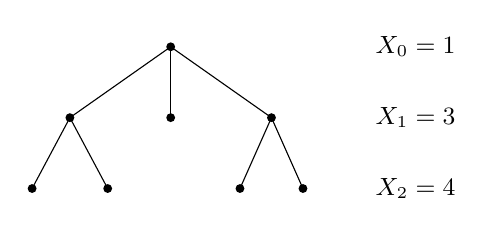
\begin{tikzpicture}[x=0.8cm, y=0.9cm]
	\coordinate (r) at (0,0);
	\coordinate (a1) at (-1.6,-1); \coordinate (a2) at (0,-1); \coordinate (a3) at (1.6,-1);
	\coordinate (b1) at (-2.2,-2); \coordinate (b2) at (-1,-2);
	\coordinate (b3) at (1.1,-2); \coordinate (b4) at (2.1,-2);
	\draw (r) -- (a1); \draw (r) -- (a2); \draw (r) -- (a3);
	\draw (a1) -- (b1); \draw (a1) -- (b2);
	\draw (a3) -- (b3); \draw (a3) -- (b4);
	\foreach \p in {r,a1,a2,a3,b1,b2,b3,b4} \fill (\p) circle (1.6pt);
	\node[right, font=\small] at (3.1,0) {$X_0 = 1$};
	\node[right, font=\small] at (3.1,-1) {$X_1 = 3$};
	\node[right, font=\small] at (3.1,-2) {$X_2 = 4$};
\end{tikzpicture}
\end{center}

\subsection{Expected Generation Size}

The first natural question to ask about a branching process is how big we expect the $n$th generation to be.

\begin{theorem}[Mean Growth]
	Let $\mu = \EE[X_1]$ be the mean of the offspring distribution. Then
	$$
	\EE[X_n] = \mu^n.
	$$
\end{theorem}
\begin{proof}
	By our random sums formula (or directly by conditioning on $X_n$ with the tower property),
	$$
	\EE[X_{n + 1}] = \EE\big[\EE[X_{n+1} \mid X_n]\big] = \EE[X_n \mu] = \mu\, \EE[X_n],
	$$
	and since $\EE[X_0] = 1$, induction gives $\EE[X_n] = \mu^n$.
\end{proof}

So in expectation the population grows or decays geometrically, with the critical threshold at $\mu = 1$. This suggests -- correctly, as we will see -- that the fate of the process hinges on whether each individual has more or less than one child on average.

\subsection{Generating Functions of Generations}

Let $G(z) = \EE[z^{X_1}]$ be the pgf of the offspring distribution, and let $G_n(z) = \EE[z^{X_n}]$ be the pgf of the $n$th generation.

\begin{theorem}[Iterating the pgf]
	For all $n \geq 0$,
	$$
	G_{n + 1}(z) = G_n(G(z)) = \underbrace{G(G(\cdots G(z) \cdots))}_{n + 1 \text{ times}}.
	$$
\end{theorem}
\begin{proof}
	Since $X_{n+1}$ is a random sum of $X_n$ independent copies of the offspring distribution, the compounding theorem gives $G_{n + 1}(z) = G_n(G(z))$ directly. Unwinding the recursion (with $G_1 = G$) shows $G_n$ is the $n$-fold iterate of $G$, and in particular the composition can be taken in either order.
\end{proof}

So the entire distributional structure of the branching process is encoded in iterating a single function -- a lovely fact, even if iterates are rarely explicitly computable.

\subsection{Extinction}

We say the process goes \vocab{extinct} if $X_n = 0$ for some $n$. Let
$$
q = \PP(\text{extinction}), \qquad q_n = \PP(X_n = 0).
$$
Since $X_n = 0$ forces $X_{n+1} = 0$, the events $\{X_n = 0\}$ are increasing, and their union is the event of extinction. So by continuity of the probability measure (finally paying off!),
$$
q_n \longrightarrow q \quad \text{as } n \rightarrow \infty.
$$
Moreover, $q_n = \PP(X_n = 0) = G_n(0)$, so the extinction probabilities are obtained by iterating $G$ starting from $0$:
$$
q_{n + 1} = G(q_n),
$$
and letting $n \rightarrow \infty$, continuity of $G$ on $[0, 1]$ gives the key equation
$$
q = G(q).
$$
So the extinction probability is a fixed point of the offspring pgf. But $G$ may have several fixed points in $[0,1]$ (note $G(1) = 1$ always!), so which one is $q$? The picture below, showing the iteration $q_{n+1} = G(q_n)$ climbing the `staircase' between the graph of $G$ and the diagonal, should be rather suggestive: starting from $q_0 = 0$, the iterates converge to the \emph{first} crossing of the curve and the diagonal.

\begin{center}
\begin{tikzpicture}[scale=4.5]
	\draw[->] (0,0) -- (1.18,0) node[right, font=\small] {$t$};
	\draw[->] (0,0) -- (0,1.18);
	\draw[dashed] (0,0) -- (1.05,1.05);
	\draw[thick, samples=100, smooth, domain=0:1, color=blue] plot (\x, {0.25 + 0.25*\x + 0.5*\x*\x});
	\draw[->] (0,0) -- (0,0.25);
	\draw[->] (0,0.25) -- (0.25,0.25);
	\draw[->] (0.25,0.25) -- (0.25,0.34375);
	\draw[->] (0.25,0.34375) -- (0.34375,0.34375);
	\draw (0.34375,0.34375) -- (0.34375,0.39465) -- (0.39465,0.39465) -- (0.39465,0.42455) -- (0.42455,0.42455) -- (0.42455,0.44379) -- (0.44379,0.44379);
	\fill (0.5,0.5) circle (0.5pt);
	\fill (1,1) circle (0.5pt);
	\draw[dashed] (0.5,0.5) -- (0.5,0);
	\node[below, font=\small] at (0.5,0) {$q$};
	\draw (1,0.012) -- (1,-0.012);
	\node[below, font=\small] at (1,0) {$1$};
	\node[left, font=\small] at (0,0.25) {$G(0)$};
\end{tikzpicture}
\end{center}

\begin{theorem}[Extinction Probability]
	The extinction probability $q$ is the \emph{smallest} non-negative solution of $G(t) = t$. Moreover, if $\PP(X_1 = 1) < 1$, then
	$$
	q < 1 \iff \mu > 1,
	$$
	where $\mu = \EE[X_1]$.
\end{theorem}
\begin{proof}
	First, minimality. Let $t \geq 0$ satisfy $G(t) = t$; we show $q_n \leq t$ for all $n$ by induction, whence $q = \lim q_n \leq t$. Indeed $q_0 = 0 \leq t$, and if $q_n \leq t$ then since $G$ has non-negative power series coefficients it is increasing on $[0, 1]$, so
	$$
	q_{n + 1} = G(q_n) \leq G(t) = t.
	$$
	Since $q$ itself solves $G(q) = q$, it must be the smallest such solution.

	Now for the criterion. Write $g_r = \PP(X_1 = r)$. If $g_0 + g_1 = 1$ (so no individual ever has two or more children) then $\mu \leq 1$; and unless $g_1 = 1$ (excluded), extinction is certain since the single line of descent dies at each step with probability $g_0 > 0$ -- consistent with the claim. So suppose $g_0 + g_1 < 1$, which makes
	$$
	G''(z) = \sum_{r \geq 2} r(r - 1)g_r z^{r - 2} > 0 \quad \text{for } z \in (0, 1),
	$$
	i.e.\ $G$ is strictly convex on $(0, 1)$. Consider $H(z) = G(z) - z$, which satisfies $H(1) = 0$ and $H(0) = g_0 \geq 0$, and is strictly convex. A strictly convex function can have at most two roots in $[0,1]$, so besides $z = 1$ there is at most one other root of $H$.

	Suppose $\mu = G'(1^-) > 1$. Then $H'(1^-) = G'(1^-) - 1 > 0$, so $H(z) < 0$ for $z$ slightly less than $1$. Since $H(0) \geq 0$ and $H$ is continuous, $H$ has a root $r \in [0, 1)$, and by minimality $q \leq r < 1$. So the process survives with positive probability.

	Conversely suppose $\mu \leq 1$. Then for $z \in (0,1)$, by strict convexity $G'(z) < G'(1^-) = \mu \leq 1$, so $H'(z) = G'(z) - 1 < 0$ on $(0, 1)$: $H$ is strictly decreasing there. Since $H(1) = 0$, we get $H(z) > 0$ for all $z \in [0, 1)$, i.e.\ there is no fixed point below $1$, and hence $q = 1$: extinction is certain.
\end{proof}

This is a genuinely striking result. If $\mu \leq 1$ the population dies out with probability $1$ -- even in the critical case $\mu = 1$ where the \emph{expected} population size stays constant forever! And if $\mu > 1$, survival is possible but by no means guaranteed: the survival probability is $1 - q$ where $q$ is the smaller fixed point.

\begin{example}
	Suppose each individual has $0$, $1$ or $2$ children with probability $\frac14, \frac14, \frac12$ respectively. Then $\mu = \frac54 > 1$, so we expect $q < 1$. The pgf is $G(z) = \frac14 + \frac14 z + \frac12 z^2$, and solving $G(t) = t$:
	$$
	\tfrac12 t^2 - \tfrac34 t + \tfrac14 = 0 \iff 2t^2 - 3t + 1 = 0 \iff (2t - 1)(t - 1) = 0,
	$$
	so $t = \frac12$ or $t = 1$. The extinction probability is the smaller root, $q = \frac{1}{2}$.
\end{example}


\section{Continuous Random Variables}

So far all of our random variables have taken countably many values. But plenty of natural quantities -- waiting times, positions, measurement errors -- vary over a continuum, and for these a new framework is needed: no pmf can describe a random variable for which every individual value has probability zero.

\subsection{Distribution Functions}

The right object to focus on turns out to be the following.

\begin{definition}[Distribution Function]
	Let $X$ be a random variable, i.e.\ a function $X: \Omega \rightarrow \R$ with $\{\omega : X(\omega) \leq x\} \in \FF$ for all $x$\footnote{Note this condition is a slight refinement of the one we used for discrete random variables -- for those, the two conditions agree.}. The \vocab{distribution function} of $X$ is
	$$
	F_X(x) = \PP(X \leq x).
	$$
\end{definition}

The distribution function makes sense for \emph{any} random variable, discrete or not, and it completely determines the distribution. Its basic properties are as follows.

\begin{proposition}[Properties of Distribution Functions]
	Let $F = F_X$ be a distribution function. Then
	\begin{enumerate}[label=(\roman*)]
		\item $F$ is non-decreasing,
		\item $\PP(a < X \leq b) = F(b) - F(a)$ for $a < b$,
		\item $F$ is right continuous, and has left limits with $F(x^-) = \PP(X < x)$,
		\item $F(x) \rightarrow 0$ as $x \rightarrow -\infty$ and $F(x) \rightarrow 1$ as $x \rightarrow \infty$.
	\end{enumerate}
\end{proposition}
\begin{proof}
	(i) follows since $\{X \leq x\} \subseteq \{X \leq y\}$ for $x \leq y$, and (ii) since $\{X \leq b\}$ is the disjoint union of $\{X \leq a\}$ and $\{a < X \leq b\}$.

	For (iii), the events $A_n = \{x < X \leq x + \frac{1}{n}\}$ are decreasing with empty intersection, so their complements are increasing with union $\Omega \backslash \bigcap_n A_n$, and continuity of $\PP$ gives $\PP(A_n) \rightarrow 0$; but $\PP(A_n) = F(x + \frac1n) - F(x)$, which together with monotonicity gives right continuity. Similarly, $B_n = \{X \leq x - \frac1n\}$ is an increasing sequence of events with union $\{X < x\}$, so $F(x - \frac1n) \rightarrow \PP(X < x)$, and monotonicity upgrades this to the full left limit. Part (iv) is another application of continuity of $\PP$, with the events $\{X \leq -n\}$ (decreasing to $\emptyset$) and $\{X \leq n\}$ (increasing to $\Omega$).
\end{proof}

For a discrete random variable, $F$ is a step function, jumping by $\PP(X = x)$ at each $x$ in the image (shown below on the left). The random variables of interest in this section sit at the other extreme, with no jumps at all (below right).

\begin{center}
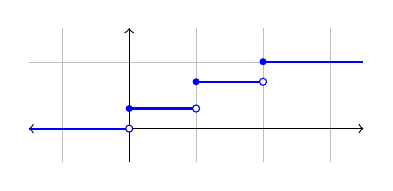
\begin{tikzpicture}[scale=0.85]
	\draw[ultra thin, color=lightgray] (-1.5,-0.5) grid (3.5,1.5);
	\draw[<->] (-1.5,0) -- (3.5,0);
	\draw[->] (0,-0.5) -- (0,1.5);
	\draw[thick, color=blue] (-1.5,0) -- (0,0);
	\draw[thick, color=blue] (0,0.3) -- (1,0.3);
	\draw[thick, color=blue] (1,0.7) -- (2,0.7);
	\draw[thick, color=blue] (2,1) -- (3.5,1);
	\draw[color=blue, fill=white] (0,0) circle (1.5pt);
	\draw[color=blue, fill=white] (1,0.3) circle (1.5pt);
	\draw[color=blue, fill=white] (2,0.7) circle (1.5pt);
	\fill[blue] (0,0.3) circle (1.5pt);
	\fill[blue] (1,0.7) circle (1.5pt);
	\fill[blue] (2,1) circle (1.5pt);
\end{tikzpicture}
\qquad
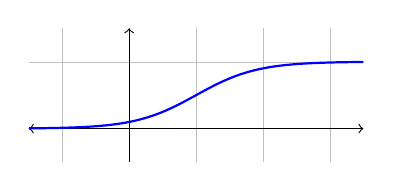
\begin{tikzpicture}[scale=0.85]
	\draw[ultra thin, color=lightgray] (-1.5,-0.5) grid (3.5,1.5);
	\draw[<->] (-1.5,0) -- (3.5,0);
	\draw[->] (0,-0.5) -- (0,1.5);
	\draw[thick, samples=100, smooth, domain=-1.5:3.5, color=blue] plot (\x, {1/(1 + exp(-2.2*(\x - 1)))});
\end{tikzpicture}
\end{center}

\begin{definition}[Continuous Random Variable]
	A random variable $X$ is \vocab{continuous} if its distribution function $F$ is continuous. In this course we work with the (slightly stronger, but much more usable) assumption that $F$ is differentiable\footnote{Strictly, such random variables are called \emph{absolutely continuous}; we will not fuss over the distinction, and `continuous random variable' will always mean this.}, and we call
	$$
	f(x) = F'(x)
	$$
	the \vocab{probability density function} (or \vocab{density}) of $X$.
\end{definition}

Note that for a continuous random variable, $\PP(X = x) = F(x) - F(x^-) = 0$ for every single $x$ -- and yet $X$ certainly takes \emph{some} value. Individual values are all negligible; only ranges of values carry probability. By the fundamental theorem of calculus,
$$
\PP(a < X \leq b) = F(b) - F(a) = \int_a^b f(x) \dd x,
$$
and more generally $\PP(X \in S) = \int_S f(x)\dd x$ for reasonable sets $S$. So the density is exactly what its name suggests: probability per unit length. For a small interval,
$$
\PP(x < X \leq x + \delta) \approx f(x)\,\delta,
$$
which is the right intuition to have -- $f(x)$ is the continuous analogue of $\PP(X = x)$, but it is not itself a probability (indeed, densities can exceed $1$!). Any density satisfies $f \geq 0$ and $\int_{-\infty}^{\infty} f(x)\dd x = 1$, and conversely any such function defines a distribution.

\subsection{Expectation and Variance}

The definition of expectation transfers from the discrete world by replacing sums with integrals (and pmfs with densities).

\begin{definition}[Expectation]
	Let $X$ be a continuous random variable with density $f$. If $X \geq 0$, we define
	$$
	\EE[X] = \int_0^{\infty} x f(x) \dd x,
	$$
	which is either finite or $+\infty$. In general, writing $X = X^+ - X^-$ with $X^+ = \max(X, 0)$ and $X^- = \max(-X, 0)$, we set $\EE[X] = \EE[X^+] - \EE[X^-] = \int_{-\infty}^{\infty} xf(x)\dd x$, provided at least one of the two parts is finite.
	\end{definition}

The expectation retains all of its old properties: it is linear, monotone, and satisfies the law of the subconscious statistician
$$
\EE[g(X)] = \int_{-\infty}^{\infty} g(x)f(x)\dd x,
$$
along with the same definitions and identities for variance and covariance as before, e.g.\ $\var(X) = \EE[X^2] - \EE[X]^2$. The tail-sum formula also survives, now in integral form.

\begin{proposition}[Tail Formula]
	If $X \geq 0$ is a continuous random variable, then
	$$
	\EE[X] = \int_0^{\infty} \PP(X \geq x) \dd x.
	$$
\end{proposition}
\begin{proof}
	We write $x = \int_0^x \dd y$ inside the definition and swap the order of integration\footnote{Justified since the integrand is non-negative (this is Fubini's theorem, or can be checked directly here).}:
	$$
	\EE[X] = \int_0^{\infty}\!\! \int_0^x \dd y \, f(x)\dd x = \int_0^{\infty}\!\! \int_y^{\infty} f(x)\dd x \dd y = \int_0^{\infty} \PP(X \geq y)\dd y. \qedhere
	$$
\end{proof}

Likewise, our inequalities (Markov, Chebyshev, Cauchy-Schwarz, Jensen) were proved using only properties of expectation, so they hold verbatim for continuous random variables.

\subsection{The Uniform and Exponential Distributions}

Let's meet the continuous analogues of the `standard' discrete distributions.

\subsubsection*{The Uniform Distribution}

The \vocab{uniform distribution} on $[a, b]$, written $X \sim \mathrm{U}[a, b]$, models a point chosen `completely at random' from the interval:
$$
f(x) = \begin{cases}
	\frac{1}{b - a} & x \in [a, b],\\
	0 & \text{otherwise},
\end{cases}
\qquad
F(x) = \frac{x - a}{b - a} \text{ for } x \in [a, b].
$$
The density (left) and distribution function (right) look as follows.

\begin{center}
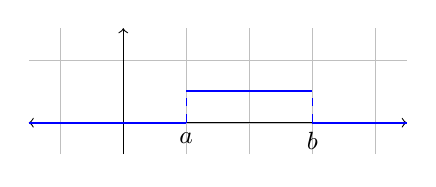
\begin{tikzpicture}[scale=0.8]
	\draw[ultra thin, color=lightgray] (-1.5,-0.5) grid (4.5,1.5);
	\draw[<->] (-1.5,0) -- (4.5,0);
	\draw[->] (0,-0.5) -- (0,1.5);
	\draw[thick, color=blue] (-1.5,0) -- (1,0);
	\draw[thick, color=blue] (1,0.5) -- (3,0.5);
	\draw[thick, color=blue] (3,0) -- (4.5,0);
	\draw[dashed, color=blue] (1,0) -- (1,0.5);
	\draw[dashed, color=blue] (3,0) -- (3,0.5);
	\node[below, font=\small] at (1,0) {$a$};
	\node[below, font=\small] at (3,0) {$b$};
\end{tikzpicture}
\qquad
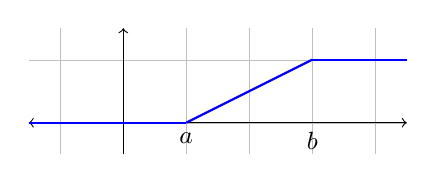
\begin{tikzpicture}[scale=0.8]
	\draw[ultra thin, color=lightgray] (-1.5,-0.5) grid (4.5,1.5);
	\draw[<->] (-1.5,0) -- (4.5,0);
	\draw[->] (0,-0.5) -- (0,1.5);
	\draw[thick, color=blue] (-1.5,0) -- (1,0);
	\draw[thick, color=blue] (1,0) -- (3,1);
	\draw[thick, color=blue] (3,1) -- (4.5,1);
	\node[below, font=\small] at (1,0) {$a$};
	\node[below, font=\small] at (3,0) {$b$};
\end{tikzpicture}
\end{center}

A quick integration gives $\EE[X] = \frac{a + b}{2}$ (no surprises), and computing $\EE[X^2] = \frac{a^2 + ab + b^2}{3}$ leads to $\var(X) = \frac{(b-a)^2}{12}$.

\subsubsection*{The Exponential Distribution}

The \vocab{exponential distribution} with rate $\lambda > 0$, written $X \sim \mathrm{Exp}(\lambda)$, has
$$
f(x) = \lambda e^{-\lambda x} \quad (x > 0), \qquad F(x) = 1 - e^{-\lambda x}.
$$
It is the continuous model of a waiting time for an event occurring `at rate $\lambda$'. The density decays exponentially (left), and the distribution function climbs towards $1$ (right); here $\lambda = 1$.

\begin{center}
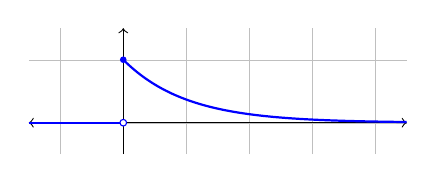
\begin{tikzpicture}[scale=0.8]
	\draw[ultra thin, color=lightgray] (-1.5,-0.5) grid (4.5,1.5);
	\draw[<->] (-1.5,0) -- (4.5,0);
	\draw[->] (0,-0.5) -- (0,1.5);
	\draw[thick, color=blue] (-1.5,0) -- (0,0);
	\draw[thick, samples=100, smooth, domain=0:4.5, color=blue] plot (\x, {exp(-\x)});
	\draw[color=blue, fill=white] (0,0) circle (1.5pt);
	\fill[blue] (0,1) circle (1.5pt);
\end{tikzpicture}
\qquad
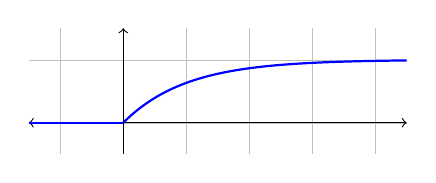
\begin{tikzpicture}[scale=0.8]
	\draw[ultra thin, color=lightgray] (-1.5,-0.5) grid (4.5,1.5);
	\draw[<->] (-1.5,0) -- (4.5,0);
	\draw[->] (0,-0.5) -- (0,1.5);
	\draw[thick, color=blue] (-1.5,0) -- (0,0);
	\draw[thick, samples=100, smooth, domain=0:4.5, color=blue] plot (\x, {1 - exp(-\x)});
\end{tikzpicture}
\end{center}

Integrating by parts (or by the tail formula, $\int_0^\infty e^{-\lambda x}\dd x$) gives
$$
\EE[X] = \frac{1}{\lambda}, \qquad \var(X) = \frac{1}{\lambda^2}.
$$
The exponential distribution should be thought of as a continuous limit of the geometric distribution: if $T \sim \mathrm{Exp}(\lambda)$ then $\lfloor nT \rfloor$ satisfies
$$
\PP(\lfloor nT \rfloor \geq k) = \PP(T \geq k/n) = \left(e^{-\lambda/n}\right)^k,
$$
which is a geometric tail with success probability $1 - e^{-\lambda/n} \approx \lambda/n$ -- checking a coin with tiny success chance many times a second.

The property that really characterises the exponential distribution is that it is \emph{memoryless}: knowing you have already waited $s$ minutes tells you nothing about how much longer you'll wait.

\begin{theorem}[Memorylessness]
	Let $T$ be a positive continuous random variable, not identically $0$ or $\infty$. Then
	$$
	\PP(T > t + s \mid T > s) = \PP(T > t) \text{ for all } s, t \geq 0
	$$
	if and only if $T \sim \mathrm{Exp}(\lambda)$ for some $\lambda > 0$.
\end{theorem}
\begin{proof}
	If $T \sim \mathrm{Exp}(\lambda)$, then
	$$
	\PP(T > t + s \mid T > s) = \frac{\PP(T > t + s)}{\PP(T > s)} = \frac{e^{-\lambda(t + s)}}{e^{-\lambda s}} = e^{-\lambda t} = \PP(T > t).
	$$
	Conversely, suppose $T$ is memoryless, and let $g(t) = \PP(T > t)$, so that $g$ satisfies the functional equation $g(t + s) = g(t)g(s)$. Then for positive integers $m, n$,
	$$
	g(m) = g(1)^m, \qquad g(m/n)^n = g(m) \implies g(m/n) = g(1)^{m/n},
	$$
	so $g(q) = g(1)^q$ for all rationals $q > 0$. Now $g(1) \in (0, 1)$: if $g(1) = 0$ then $g(q) = 0$ for all rational $q > 0$ and $T = 0$ almost surely; if $g(1) = 1$ then similarly $T = \infty$ almost surely -- both excluded. So we may define $\lambda = -\log g(1) > 0$, giving $g(q) = e^{-\lambda q}$ on the rationals. Finally, $g$ is decreasing, so for real $t$, squeezing $t$ between rationals $r \leq t \leq s$ with $s - r$ small gives $e^{-\lambda s} \leq g(t) \leq e^{-\lambda r}$, and hence $g(t) = e^{-\lambda t}$ everywhere.
\end{proof}

\subsection{The Normal Distribution}

We now come to the most important distribution in all of probability -- the reason for its ubiquity being the central limit theorem, which we will meet in due course.

\begin{definition}[Normal Distribution]
	The \vocab{normal} (or \vocab{Gaussian}) \vocab{distribution} with mean $\mu \in \R$ and variance $\sigma^2 > 0$, written $N(\mu, \sigma^2)$, has density
	$$
	f(x) = \frac{1}{\sqrt{2\pi \sigma^2}} \exp\left(-\frac{(x - \mu)^2}{2\sigma^2}\right), \quad x \in \R.
	$$
	The case $N(0, 1)$ is called the \vocab{standard normal distribution}, and its distribution function is denoted $\Phi$, with density $\phi(x) = \frac{1}{\sqrt{2\pi}}e^{-x^2/2}$.
\end{definition}

The density is the famous `bell curve', symmetric about $\mu$, with the standard deviation $\sigma$ setting the width of the bell ($\mu \pm \sigma$ are precisely its points of inflection):

\begin{center}
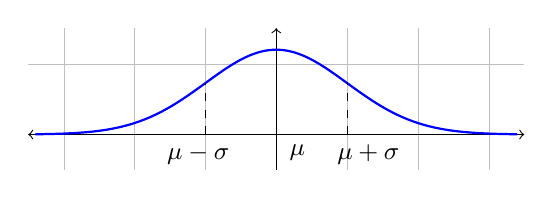
\begin{tikzpicture}[scale=0.9]
	\draw[ultra thin, color=lightgray] (-3.5,-0.5) grid (3.5,1.5);
	\draw[<->] (-3.5,0) -- (3.5,0);
	\draw[->] (0,-0.5) -- (0,1.5);
	\draw[thick, samples=100, smooth, domain=-3.4:3.4, color=blue] plot (\x, {3*exp(-\x*\x/2)/sqrt(2*pi)});
	\draw[dashed] (-1,0) -- (-1,{3*exp(-0.5)/sqrt(2*pi)});
	\draw[dashed] (1,0) -- (1,{3*exp(-0.5)/sqrt(2*pi)});
	\node[below, font=\small] at (-1.1,0) {$\mu - \sigma$};
	\node[below right, font=\small] at (0.05,0) {$\mu$};
	\node[below, font=\small] at (1.3,0) {$\mu + \sigma$};
\end{tikzpicture}
\end{center}

We should first check that this is actually a density -- the source of the mysterious $\sqrt{2\pi}$.

\begin{proposition}
	$\displaystyle\int_{-\infty}^{\infty} \frac{1}{\sqrt{2\pi\sigma^2}} \exp\left(-\frac{(x-\mu)^2}{2\sigma^2}\right)\dd x = 1$.
\end{proposition}
\begin{proof}
	Substituting $u = (x - \mu)/\sigma$ reduces to showing $I = \int_{-\infty}^{\infty} e^{-u^2/2}\dd u = \sqrt{2\pi}$. We use the famous squaring trick: writing $I^2$ as a double integral and changing to polar coordinates $(u, v) = (r\cos\theta, r\sin\theta)$,
	$$
	I^2 = \int_{-\infty}^{\infty}\!\int_{-\infty}^{\infty} e^{-(u^2 + v^2)/2}\dd u \dd v = \int_0^{2\pi}\!\!\int_0^{\infty} e^{-r^2/2}\, r\dd r\dd\theta = 2\pi \left[-e^{-r^2/2}\right]_0^{\infty} = 2\pi,
	$$
	and since $I > 0$ we get $I = \sqrt{2\pi}$.
\end{proof}

The parameters deserve their names: if $X \sim N(\mu, \sigma^2)$ then
$$
\EE[X] = \int_{-\infty}^{\infty} \frac{x - \mu}{\sqrt{2\pi\sigma^2}}e^{-(x - \mu)^2/2\sigma^2}\dd x + \mu = 0 + \mu = \mu,
$$
the first integral vanishing since the integrand is odd about $\mu$; and substituting $u = (x - \mu)/\sigma$ and integrating by parts,
$$
\var(X) = \sigma^2 \int_{-\infty}^{\infty} \frac{u^2}{\sqrt{2\pi}}e^{-u^2/2}\dd u = \sigma^2.
$$
Also note the symmetry $\phi(x) = \phi(-x)$, which gives the frequently-used relation $\Phi(-x) = 1 - \Phi(x)$.

\subsection{Transformations of Random Variables}

Given a random variable $X$ with known density and a function $g$, what is the density of $g(X)$? For monotone $g$ there is a clean answer, and the proof is simply `differentiate the distribution function'.

\begin{theorem}[Densities Under Monotone Maps]
	Let $X$ be a continuous random variable with density $f$, and let $g$ be strictly monotone with differentiable inverse. Then $Y = g(X)$ is a continuous random variable with density
	$$
	f_Y(y) = f\big(g^{-1}(y)\big) \left|\frac{\mathrm{d}}{\mathrm{d}y} g^{-1}(y)\right|.
	$$
\end{theorem}
\begin{proof}
	Suppose first that $g$ is strictly increasing. Then $g(X) \leq y \iff X \leq g^{-1}(y)$, so
	$$
	F_Y(y) = \PP(g(X) \leq y) = F\big(g^{-1}(y)\big),
	$$
	and differentiating with the chain rule gives $f_Y(y) = f(g^{-1}(y)) \cdot (g^{-1})'(y)$, where the derivative is positive. If instead $g$ is strictly decreasing, then $g(X) \leq y \iff X \geq g^{-1}(y)$, so $F_Y(y) = 1 - F(g^{-1}(y))$, and differentiating gives $f_Y(y) = f(g^{-1}(y)) \cdot \left(-(g^{-1})'(y)\right)$, where now $-(g^{-1})' = |(g^{-1})'|$. Both cases match the claimed formula.
\end{proof}

Rather than memorising this, it is usually safer to redo the two-line calculation with distribution functions -- but the formula gives an important structural fact about the normal family.

\begin{corollary}[Linear Maps of Normals]
	If $X \sim N(\mu, \sigma^2)$ and $a \neq 0, b \in \R$, then
	$$
	aX + b \sim N(a\mu + b, a^2\sigma^2).
	$$
	In particular, $(X - \mu)/\sigma \sim N(0,1)$.
\end{corollary}
\begin{proof}
	Applying the theorem with $g(x) = ax + b$, so $g^{-1}(y) = (y - b)/a$,
	$$
	f_Y(y) = \frac{1}{\sqrt{2\pi\sigma^2}}\exp\left(-\frac{(\frac{y - b}{a} - \mu)^2}{2\sigma^2}\right)\cdot\frac{1}{|a|} = \frac{1}{\sqrt{2\pi a^2\sigma^2}}\exp\left(-\frac{(y - (a\mu + b))^2}{2a^2\sigma^2}\right),
	$$
	which is the $N(a\mu + b, a^2\sigma^2)$ density.
\end{proof}

The process of passing from $X$ to $(X - \mu)/\sigma$ is called \emph{standardisation}, and is how one uses tables of $\Phi$ in practice: every question about a normal random variable reduces to one about the standard normal.


\section{Joint Densities}

Just as in the discrete setting, the interesting questions about continuous random variables involve several of them at once, and for this we need joint densities.

\subsection{Joint Densities and Independence}

Just as in the discrete setting, understanding several continuous random variables at once means studying their joint behaviour.

\begin{definition}[Joint Density]
	Random variables $X_1, \dots, X_n$ have \vocab{joint density} $f: \R^n \rightarrow [0, \infty)$ if
	$$
	\PP(X_1 \leq x_1, \dots, X_n \leq x_n) = \int_{-\infty}^{x_1} \!\!\cdots \int_{-\infty}^{x_n} f(y_1, \dots, y_n) \dd y_1 \cdots \dd y_n
	$$
	for all $x_1, \dots, x_n \in \R$.
\end{definition}

As before, this extends to $\PP((X_1, \dots, X_n) \in B) = \int_B f$ for reasonable sets $B \subseteq \R^n$, and the density can be recovered by (partial) differentiation of the joint distribution function. The density of a single coordinate, called its \vocab{marginal density}, is obtained by integrating out the others:
$$
f_{X_1}(x_1) = \int_{-\infty}^{\infty}\!\!\cdots\int_{-\infty}^{\infty} f(x_1, y_2, \dots, y_n) \dd y_2 \cdots \dd y_n.
$$

For independence, we can no longer compare with products of point probabilities (they're all zero!), so we phrase everything in terms of distribution functions: $X_1, \dots, X_n$ are \vocab{independent} if
$$
\PP(X_1 \leq x_1, \dots, X_n \leq x_n) = \PP(X_1 \leq x_1) \cdots \PP(X_n \leq x_n) \quad \text{for all } x_i.
$$
The key practical criterion is that independence corresponds exactly to the joint density factorising.

\begin{theorem}[Factorisation Criterion]
	Suppose $(X_1, \dots, X_n)$ has joint density $f$.
	\begin{enumerate}[label=(\roman*)]
		\item If $X_1, \dots, X_n$ are independent with marginal densities $f_1, \dots, f_n$, then
		$$
		f(x_1, \dots, x_n) = f_1(x_1)\cdots f_n(x_n).
		$$
		\item Conversely, if $f(x_1, \dots, x_n) = g_1(x_1) \cdots g_n(x_n)$ for some non-negative functions $g_i$, then the $X_i$ are independent, with densities proportional to the $g_i$.
	\end{enumerate}
\end{theorem}
\begin{proof}
	For (i), independence lets us factor the joint distribution function into $\prod_i \int_{-\infty}^{x_i} f_i$, which is precisely the statement that $\prod_i f_i$ serves as a joint density.

	For (ii), let $c_i = \int_{-\infty}^{\infty} g_i(y)\dd y$. Since $f$ integrates to $1$ over $\R^n$, we get $c_1 c_2 \cdots c_n = 1$. Now integrating out all variables except the $i$th shows the marginal density of $X_i$ is $g_i \cdot \prod_{j \neq i} c_j = g_i / c_i$. Then
	$$
	\PP(X_1 \leq x_1, \dots, X_n \leq x_n) = \prod_{i} \int_{-\infty}^{x_i} g_i(y_i) \dd y_i = \prod_i \int_{-\infty}^{x_i} \frac{g_i(y_i)}{c_i}\dd y_i = \prod_i \PP(X_i \leq x_i),
	$$
	using $\prod_i c_i = 1$, so the $X_i$ are independent with the claimed densities.
\end{proof}

\subsection{Sums of Continuous Random Variables}

The distribution of a sum of independent continuous random variables is again given by a convolution, with the sum over values replaced by an integral.

\begin{proposition}[Convolution]
	Let $X$ and $Y$ be independent with densities $f_X$ and $f_Y$. Then $X + Y$ has density
	$$
	f_{X + Y}(z) = \int_{-\infty}^{\infty} f_X(x) f_Y(z - x) \dd x.
	$$
\end{proposition}
\begin{proof}
	We compute the distribution function of the sum by integrating the joint density $f_X(x)f_Y(y)$ over the half plane $\{x + y \leq z\}$:
	$$
	\PP(X + Y \leq z) = \int_{-\infty}^{\infty} \!\!\int_{-\infty}^{z - x} f_X(x)f_Y(y)\dd y \dd x = \int_{-\infty}^{z}\left(\int_{-\infty}^{\infty} f_X(x)f_Y(u - x)\dd x \right)\dd u,
	$$
	substituting $u = y + x$ in the inner integral and then swapping the order of integration. The result is the integral up to $z$ of the claimed density, which proves the claim.
\end{proof}

\subsection{Conditional Densities}

Conditioning on the value of a continuous random variable looks dangerous -- the conditioning event $\{Y = y\}$ has probability zero -- but at the level of densities everything goes through smoothly.

\begin{definition}[Conditional Density]
	Let $X, Y$ have joint density $f_{X, Y}$, and let $y$ be such that $f_Y(y) > 0$. The \vocab{conditional density of $X$ given $Y = y$} is
	$$
	f_{X \mid Y}(x \mid y) = \frac{f_{X, Y}(x, y)}{f_Y(y)}.
	$$
\end{definition}

This is the exact analogue of $\PP(X = x \mid Y = y)$, and one can justify it by conditioning on the event $\{y < Y \leq y + \delta\}$ and letting $\delta \rightarrow 0$. Integrating out the conditioning value gives the continuous law of total probability,
$$
f_X(x) = \int_{-\infty}^{\infty} f_{X \mid Y}(x \mid y) f_Y(y) \dd y,
$$
and we can define conditional expectation just as before: $\EE[X \mid Y] = g(Y)$ where
$$
g(y) = \int_{-\infty}^{\infty} x \, f_{X \mid Y}(x \mid y)\dd x.
$$
All the properties from the discrete case (linearity, the tower property, taking out what is known) continue to hold.

\subsection{Transformations in Higher Dimensions}

The change of variables formula for densities generalises to $\R^d$, with the derivative replaced by a Jacobian determinant -- exactly mirroring the change of variables formula for multiple integrals.

\begin{theorem}[Multidimensional Change of Variables]
	Let $X$ be a random variable with values in $D \subseteq \R^d$ and density $f_X$, and let $g: D \rightarrow g(D)$ be a bijection with continuous derivative and $\det g'(x) \neq 0$ on $D$. Then $Y = g(X)$ has density
	$$
	f_Y(y) = f_X\big(g^{-1}(y)\big) \, |J|, \quad \text{where } J = \det\left(\frac{\partial x_i}{\partial y_j}\right)_{i, j}
	$$
	is the Jacobian of the inverse map $x = g^{-1}(y)$.
\end{theorem}

We won't prove this (it is essentially the substitution rule for multiple integrals, which we take on trust from Vector Calculus), but let's see it in action on a genuinely useful example.

\begin{example}[Polar Coordinates of a Gaussian Pair]
	Let $X, Y$ be independent standard normals, and let $(R, \Theta)$ be the polar coordinates of the point $(X, Y)$, so $X = R\cos\Theta$ and $Y = R\sin\Theta$. The Jacobian of the map $(r, \theta) \mapsto (r\cos\theta, r\sin\theta)$ is
	$$
	J = \det \begin{pmatrix}
		\cos\theta & -r\sin\theta \\ \sin\theta & r \cos\theta
	\end{pmatrix} = r,
	$$
	which is geometrically just the statement that a small `polar rectangle' with sides $\dd r$ and $r \dd\theta$ has area $r \dd r \dd \theta$:
	\begin{center}
	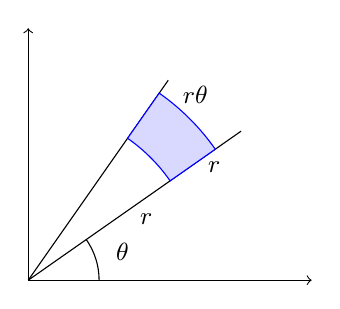
\begin{tikzpicture}[scale=1.0]
		\draw[->] (0,0) -- (3.6,0);
		\draw[->] (0,0) -- (0,3.2);
		\draw (0,0) -- (35:3.3);
		\draw (0,0) -- (55:3.1);
		\path[fill=blue!15] (35:2.2) arc (35:55:2.2) -- (55:2.9) arc (55:35:2.9) -- cycle;
		\draw[color=blue] (35:2.2) arc (35:55:2.2) -- (55:2.9) arc (55:35:2.9) -- cycle;
		\draw (0.9,0) arc (0:35:0.9);
		\node[font=\small] at (17:1.25) {$\theta$};
		\node[font=\small] at (1.5,0.78) {$r$};
		\node[font=\small, anchor=west] at (2.16,1.44) {$\dd r$};
		\node[font=\small, anchor=south] at (45:3.0) {$r \dd\theta$};
	\end{tikzpicture}
	\end{center}
	So for $r > 0$ and $\theta \in [0, 2\pi)$,
	$$
	f_{R, \Theta}(r, \theta) = f_{X,Y}(r\cos\theta, r\sin\theta) \cdot r = \frac{1}{2\pi} r e^{-r^2/2} = \underbrace{\frac{1}{2\pi}}_{f_\Theta(\theta)} \cdot \underbrace{r e^{-r^2/2}}_{f_R(r)}.
	$$
	The joint density factorises, so by the factorisation criterion $R$ and $\Theta$ are \emph{independent}, with $\Theta \sim \mathrm{U}[0, 2\pi)$ and $R$ having density $re^{-r^2/2}$. (Run backwards, this observation is a practical recipe for generating normal random variables -- the `Box-Muller' method -- which we will return to at the end of these notes.)
\end{example}

\subsection{Order Statistics}

Given independent identically distributed random variables $X_1, \dots, X_n$, we often care about their sorted values -- the smallest, the largest, the median. Sorting them into increasing order gives the \vocab{order statistics}
$$
Y_1 = X_{(1)} \leq Y_2 = X_{(2)} \leq \cdots \leq Y_n = X_{(n)}.
$$
For instance, with $n = 5$ the picture might be as follows -- the samples $X_i$ land in some scattered order on the line, and the order statistics simply relabel them from left to right.
\begin{center}
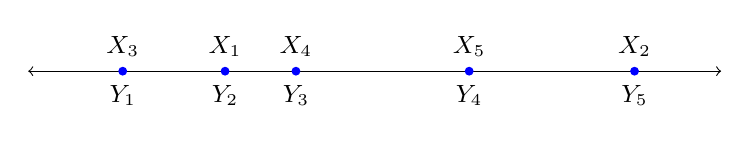
\begin{tikzpicture}[x=1cm]
	\draw[<->] (-0.4,0) -- (8.4,0);
	\foreach \x/\l/\s in {0.8/1/3, 2.1/2/1, 3.0/3/4, 5.2/4/5, 7.3/5/2} {
		\fill[blue] (\x,0) circle (1.6pt);
		\node[below, font=\small] at (\x,-0.06) {$Y_{\l}$};
		\node[above, font=\small] at (\x,0.06) {$X_{\s}$};
	}
\end{tikzpicture}
\end{center}
Suppose the $X_i$ have distribution function $F$ and density $f$. The extremes are easy to handle directly:
\begin{align*}
	\PP(Y_n \leq x) &= \PP(X_1 \leq x, \dots, X_n \leq x) = F(x)^n, \\
	\PP(Y_1 \leq x) &= 1 - \PP(X_1 > x, \dots, X_n > x) = 1 - (1 - F(x))^n,
\end{align*}
using independence, and differentiating gives their densities
$$
f_{Y_n}(x) = nF(x)^{n - 1}f(x), \qquad f_{Y_1}(x) = n(1 - F(x))^{n-1} f(x).
$$
For the full joint behaviour, we have the following.

\begin{proposition}[Joint Density of Order Statistics]
	The order statistics $(Y_1, \dots, Y_n)$ have joint density
	$$
	f_{Y_1, \dots, Y_n}(x_1, \dots, x_n) = \begin{cases}
		n! \, f(x_1) \cdots f(x_n) & \text{if } x_1 < x_2 < \cdots < x_n, \\
		0 & \text{otherwise.}
	\end{cases}
	$$
\end{proposition}
\begin{proof}
	For $x_1 < \cdots < x_n$, the event $\{Y_1 \leq x_1, \dots, Y_n \leq x_n\}$ splits according to which of the $X_i$ lands in which position of the ordering; since the $X_i$ are independent and identically distributed (and ties have probability zero), each of the $n!$ orderings contributes equally, and so
	$$
	\PP(Y_1 \leq x_1, \dots, Y_n \leq x_n) = n! \,\PP(X_1 \leq x_1, \dots, X_n \leq x_n, \, X_1 < X_2 < \cdots < X_n).
	$$
	Writing the right hand side as an integral of $f(u_1)\cdots f(u_n)$ over the region $\{u_1 \leq x_1, \dots, u_n \leq x_n,\ u_1 < \cdots < u_n\}$ and differentiating in each variable gives the claimed density.
\end{proof}

Note the factor $n!$ and the ordering constraint: the joint density does \emph{not} factorise, so the order statistics are certainly not independent (knowing the minimum is large forces the maximum to be larger still). For the exponential distribution, though, something special happens with the \emph{gaps}.

\begin{example}[Exponential Spacings]
	Let $X_1, \dots, X_n$ be independent $\mathrm{Exp}(\lambda)$, with order statistics $Y_1 \leq \cdots \leq Y_n$, and consider the spacings $Z_1 = Y_1$ and $Z_i = Y_i - Y_{i - 1}$ for $i \geq 2$. The map from $(y_1, \dots, y_n)$ to $(z_1, \dots, z_n)$ is linear with determinant $1$, and $y_i = z_1 + \cdots + z_i$, so
	\begin{align*}
		f_{Z_1, \dots, Z_n}(z_1, \dots, z_n) &= n!\, \lambda^n e^{-\lambda(y_1 + \cdots + y_n)} = n!\,\lambda^n e^{-\lambda(nz_1 + (n-1)z_2 + \cdots + z_n)} \\
		&= \prod_{i = 1}^{n} (n - i + 1)\lambda \, e^{-(n - i + 1)\lambda z_i}.
	\end{align*}
	The joint density factorises! So the spacings are independent, with $Z_i \sim \mathrm{Exp}((n - i + 1)\lambda)$. This is really memorylessness at work: when $i - 1$ of the clocks have rung, the remaining $n - i + 1$ have (conditionally) fresh exponential lifetimes, and the minimum of $k$ independent $\mathrm{Exp}(\lambda)$ variables is $\mathrm{Exp}(k\lambda)$ -- a fact worth checking directly:
	$$
	\PP(\min(X_1, \dots, X_k) > z) = \prod_{i=1}^k \PP(X_i > z) = e^{-k\lambda z}.
	$$
\end{example}


\section{Moment Generating Functions}

Probability generating functions served us wonderfully for random variables with values in $\{0, 1, 2, \dots\}$, but they make no sense for continuous random variables. The right generalisation is to replace $z^X$ with $e^{\theta X}$.

\begin{definition}[Moment Generating Function]
	The \vocab{moment generating function} (or \vocab{mgf}) of a random variable $X$ is
	$$
	m(\theta) = \EE\left[e^{\theta X}\right],
	$$
	defined for those $\theta \in \R$ where the expectation is finite. For a continuous random variable with density $f$, this is $\int_{-\infty}^{\infty} e^{\theta x}f(x)\dd x$.
\end{definition}

Note $m(0) = 1$ always, but the mgf may well be infinite for every other $\theta$, in which case it's useless. The good situation is when $m$ is finite on an open interval around $0$; then the mgf shares the two crucial properties of the pgf. The first we must take on trust (its proof needs tools beyond this course).

\begin{theorem}[Uniqueness]
	If the moment generating function of $X$ is finite on some open interval containing $0$, then it uniquely determines the distribution of $X$.
\end{theorem}

\begin{theorem}[Moments From the mgf]
	If $m$ is finite on an open interval around $0$, then for each $r \geq 0$,
	$$
	m^{(r)}(0) = \EE[X^r].
	$$
\end{theorem}

The idea behind the second result is simply to expand $e^{\theta X} = \sum_k \theta^k X^k / k!$ and differentiate term by term (the finiteness assumption is what justifies the exchanges of limits) -- so the mgf is precisely the exponential generating function of the moments, whence the name. And as with pgfs, independence turns sums into products:

\begin{theorem}[mgfs of Sums]
	If $X_1, \dots, X_n$ are independent, then
	$$
	\EE\left[e^{\theta(X_1 + \cdots + X_n)}\right] = \prod_{i = 1}^{n} \EE\left[e^{\theta X_i}\right].
	$$
\end{theorem}
\begin{proof}
	The random variables $e^{\theta X_i}$ are independent, so the expectation of their product factorises.
\end{proof}

\subsection{Examples: Gamma, Normal, and a Warning}

Let's put moment generating functions to work on some concrete distributions.

\begin{example}[The Gamma Distribution]
	The \vocab{gamma distribution} $\Gamma(n, \lambda)$, for $n \in \N$ and $\lambda > 0$, has density
	$$
	f(x) = e^{-\lambda x}\frac{\lambda^n x^{n - 1}}{(n-1)!}, \quad x > 0.
	$$
	(One checks this integrates to 1 by repeated integration by parts, reducing to the exponential case $n = 1$: indeed $\Gamma(1, \lambda) = \mathrm{Exp}(\lambda)$.) For $\theta < \lambda$, the mgf is
	\begin{align*}
		m(\theta) = \int_0^{\infty} e^{\theta x}e^{-\lambda x}\frac{\lambda^n x^{n-1}}{(n-1)!}\dd x &= \left(\frac{\lambda}{\lambda - \theta}\right)^n \int_0^{\infty} e^{-(\lambda - \theta)x}\frac{(\lambda - \theta)^n x^{n - 1}}{(n-1)!}\dd x \\
		&= \left(\frac{\lambda}{\lambda - \theta}\right)^n,
	\end{align*}
	since the final integrand is the $\Gamma(n, \lambda - \theta)$ density. (For $\theta \geq \lambda$ the integral diverges, but finiteness on $(-\infty, \lambda)$ is plenty.) Multiplying mgfs, we conclude that if $X \sim \Gamma(n, \lambda)$ and $Y \sim \Gamma(m, \lambda)$ are independent then $X + Y \sim \Gamma(n + m, \lambda)$; in particular, a sum of $n$ independent $\mathrm{Exp}(\lambda)$ waiting times has the $\Gamma(n, \lambda)$ distribution.
\end{example}

\begin{example}[The Normal Distribution]
	Let $X \sim N(\mu, \sigma^2)$. Completing the square in the exponent,
	$$
	\theta x - \frac{(x - \mu)^2}{2\sigma^2} = \theta\mu + \frac{\theta^2\sigma^2}{2} - \frac{\left(x - (\mu + \theta\sigma^2)\right)^2}{2\sigma^2},
	$$
	so
	$$
	m(\theta) = \exp\left(\theta\mu + \frac{\theta^2\sigma^2}{2}\right)\int_{-\infty}^{\infty} \frac{1}{\sqrt{2\pi\sigma^2}}\exp\left(-\frac{(x - (\mu + \theta\sigma^2))^2}{2\sigma^2}\right)\dd x = e^{\theta\mu + \theta^2\sigma^2/2},
	$$
	the integral being that of the $N(\mu + \theta\sigma^2, \sigma^2)$ density. This mgf is finite for \emph{all} $\theta$ -- the normal distribution has very thin tails. As an immediate payoff, if $X \sim N(\mu, \sigma^2)$ and $Y \sim N(\nu, \tau^2)$ are independent then
	$$
	\EE[e^{\theta(X + Y)}] = e^{\theta\mu + \theta^2\sigma^2/2}\, e^{\theta\nu + \theta^2\tau^2/2} = e^{\theta(\mu + \nu) + \theta^2(\sigma^2 + \tau^2)/2},
	$$
	so $X + Y \sim N(\mu + \nu, \sigma^2 + \tau^2)$: sums of independent normals are normal.
\end{example}

\begin{example}[The Cauchy Distribution -- A Warning]
	The \vocab{Cauchy distribution} has density
	$$
	f(x) = \frac{1}{\pi(1 + x^2)}, \quad x \in \R.
	$$
	Its tails decay so slowly that $\EE[e^{\theta X}] = \infty$ for every $\theta \neq 0$ -- indeed even $\EE[X]$ fails to exist. So mgfs tell us nothing here: $X$ and $2X$ have identical mgfs but different distributions. The moral is that all the mgf machinery genuinely requires finiteness on an open interval.
\end{example}

\section{The Central Limit Theorem}

We have arrived at the crown jewel of the course. The weak law of large numbers says the sample mean $S_n / n$ concentrates around $\mu$; the central limit theorem describes, with remarkable precision, the \emph{shape} of the fluctuations around $\mu$ -- and the answer is universal: whatever distribution you start with, the fluctuations look normal.

First, we need to say what it means for distributions to converge.

\begin{definition}[Convergence in Distribution]
	Random variables $X_n$ \vocab{converge in distribution} to $X$, written $X_n \rightarrow X$ in distribution, if
	$$
	F_{X_n}(x) \longrightarrow F_X(x) \quad \text{as } n \rightarrow \infty
	$$
	for every $x \in \R$ at which $F_X$ is continuous.
\end{definition}

(The restriction to continuity points is a technicality that avoids silly counterexamples with point masses; for a continuous limit like the normal distribution, it is no restriction at all.) The bridge between mgfs and convergence in distribution is the following theorem, which we state without proof.

\begin{theorem}[Continuity Theorem]
	Let $X$ have mgf $m$, finite on an open interval around $0$, and let $X_n$ have mgfs $m_n$. If $m_n(\theta) \rightarrow m(\theta)$ for all $\theta$, then $X_n \rightarrow X$ in distribution.
\end{theorem}

With this in hand, the central limit theorem is within reach.

\begin{theorem}[Central Limit Theorem]
	Let $X_1, X_2, \dots$ be independent identically distributed random variables with mean $\mu$ and variance $\sigma^2 \in (0, \infty)$, and let $S_n = X_1 + \cdots + X_n$. Then for every $x \in \R$,
	$$
	\PP\left(\frac{S_n - n\mu}{\sigma\sqrt{n}} \leq x \right) \longrightarrow \Phi(x) = \int_{-\infty}^{x} \frac{1}{\sqrt{2\pi}}e^{-y^2/2}\dd y \quad \text{as } n \rightarrow \infty.
	$$
	That is, $(S_n - n\mu)/\sigma\sqrt{n} \rightarrow N(0,1)$ in distribution.
\end{theorem}

Note the choice of scaling: $S_n - n\mu$ has variance $n\sigma^2$, so dividing by $\sigma\sqrt{n}$ is exactly what's needed to stabilise the fluctuations at unit size. Informally, the theorem says
$$
S_n \approx n\mu + \sigma\sqrt{n}\, Z, \quad Z \sim N(0, 1),
$$
for large $n$: the sum is its mean, plus a normal fluctuation of order $\sqrt{n}$.

\begin{proof}[Proof (assuming an mgf exists)]
	We give the proof under the additional assumption that the mgf of $X_1$ is finite on an open interval around $0$ -- this is how the result is proved in this course, and covers all the standard distributions; the general case requires characteristic functions.

	By replacing $X_i$ with $(X_i - \mu)/\sigma$, we may assume $\mu = 0$ and $\sigma = 1$, and must show $S_n/\sqrt{n} \rightarrow N(0, 1)$ in distribution. Let $m(\theta) = \EE[e^{\theta X_1}]$. By independence,
	$$
	\EE\left[e^{\theta S_n / \sqrt{n}}\right] = \prod_{i = 1}^{n}\EE\left[e^{(\theta/\sqrt{n})X_i}\right] = m\left(\frac{\theta}{\sqrt{n}}\right)^{n},
	$$
	so by the continuity theorem it suffices to show that for each fixed $\theta$,
	$$
	m\left(\frac{\theta}{\sqrt{n}}\right)^{n} \longrightarrow e^{\theta^2/2} = \EE[e^{\theta Z}].
	$$
	Since $m$ is finite near $0$, it has derivatives of all orders at $0$ given by the moments, and Taylor's theorem gives, as $t \rightarrow 0$,
	$$
	m(t) = 1 + t\,\EE[X_1] + \frac{t^2}{2}\EE[X_1^2] + o(t^2) = 1 + \frac{t^2}{2} + o(t^2),
	$$
	using $\EE[X_1] = 0$ and $\EE[X_1^2] = \var(X_1) = 1$. Applying this with $t = \theta/\sqrt{n}$,
	$$
	m\left(\frac{\theta}{\sqrt{n}}\right)^n = \left(1 + \frac{\theta^2}{2n} + o\left(\frac1n\right)\right)^{n},
	$$
	and taking logarithms, $n \log\left(1 + \frac{\theta^2}{2n} + o(\frac1n)\right) = \frac{\theta^2}{2} + o(1) \rightarrow \frac{\theta^2}{2}$, using $\log(1 + u) = u + o(u)$. So $m(\theta/\sqrt{n})^n \rightarrow e^{\theta^2/2}$, completing the proof.
\end{proof}

The really remarkable feature is \emph{universality}: the limit doesn't remember anything about the distribution of the $X_i$ except its mean and variance. This is why the normal distribution is everywhere -- any quantity that is a sum of many small independent contributions (measurement errors, say, or heights in a population) should be approximately normally distributed.

\subsection{Applications}

The real value of the central limit theorem is as an approximation tool, so let's see it in action.

\begin{example}[Normal Approximation to the Binomial]
	If $S_n \sim \mathrm{Bin}(n, p)$, then $S_n$ is a sum of $n$ independent Bernoulli variables, so by the CLT
	$$
	\frac{S_n - np}{\sqrt{np(1-p)}} \approx N(0, 1), \quad \text{i.e.} \quad S_n \approx N\big(np, np(1-p)\big)
	$$
	for large $n$. The picture below shows the pmf of $\mathrm{Bin}(16, \frac12)$ with the approximating $N(8, 4)$ density drawn over it -- the fit is already rather good.
	\begin{center}
	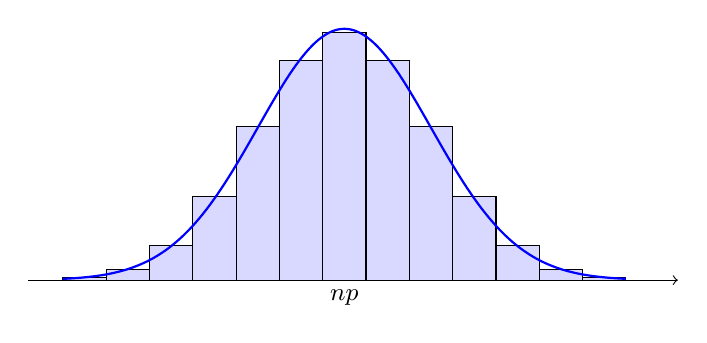
\begin{tikzpicture}[xscale=0.55, yscale=16]
		\foreach \k/\h in {2/0.0018, 3/0.0085, 4/0.0278, 5/0.0666, 6/0.1222, 7/0.1746, 8/0.1964, 9/0.1746, 10/0.1222, 11/0.0666, 12/0.0278, 13/0.0085, 14/0.0018}
			\draw[fill=blue!15, thin] (\k - 0.5, 0) rectangle (\k + 0.5, \h);
		\draw[->] (0.7,0) -- (15.7,0);
		\draw[thick, samples=100, smooth, domain=1.5:14.5, color=blue] plot (\x, {0.19947*exp(-(\x - 8)*(\x - 8)/8)});
		\node[below, font=\small] at (8,0) {$np$};
	\end{tikzpicture}
	\end{center}
	Note the contrast with the Poisson approximation: there we let $p = \lambda/n$ shrink as $n$ grew (so the CLT does not apply -- the summands change with $n$), whereas here $p$ is fixed. The rough rule: rare events give Poisson, common events give normal. Similarly, $\mathrm{Poisson}(n)$ is a sum of $n$ independent $\mathrm{Poisson}(1)$ variables, so $\mathrm{Poisson}(n) \approx N(n, n)$ for large $n$.
\end{example}

\begin{example}[Opinion Polling]
	Suppose each member of a large population independently supports a proposition with unknown probability $p$, and we poll $N$ random individuals, estimating $p$ by $\hat{p}_N = S_N/N$ where $S_N \sim \mathrm{Bin}(N, p)$. How large must $N$ be so that $|\hat p_N - p| \leq 0.04$ with probability at least $0.99$?

	By the CLT, $\hat{p}_N \approx p + \sqrt{p(1-p)/N}\, Z$ with $Z \sim N(0,1)$, so we need
	$$
	\PP\left(\sqrt{\frac{p(1-p)}{N}}\,|Z| \leq 0.04\right) \geq 0.99.
	$$
	From tables, $\PP(|Z| \leq 2.58) = 0.99$, so we require $0.04\sqrt{N/p(1-p)} \geq 2.58$. The worst case is $p = \frac12$ (maximising $p(1-p) = \frac14$), giving
	$$
	N \geq \frac{2.58^2}{4 \times 0.04^2} \approx 1040.
	$$
	Only about a thousand people -- regardless of the size of the population! The $1/\sqrt{N}$ decay of sampling error is entirely responsible for the feasibility of opinion polling.
\end{example}


\section{The Multivariate Normal Distribution}

Given how central the normal distribution is, we should understand its multidimensional version -- both because it arises in its own right (via a multidimensional CLT), and because it has some genuinely special structure not shared by other distributions.

In this section vectors are columns, and we write $u^\top$ for the transpose.

\subsection{Gaussian Vectors}

We begin by pinning down exactly what it means for a whole vector of random variables to be normally distributed.

\begin{definition}[Gaussian Vector]
	A random vector $X = (X_1, \dots, X_n)^\top$ is a \vocab{Gaussian vector} (or \vocab{multivariate normal}) if for every $u \in \R^n$, the scalar random variable
	$$
	u^\top X = u_1 X_1 + \cdots + u_n X_n
	$$
	is normally distributed (where we allow degenerate `normals' of zero variance, i.e.\ constants).
\end{definition}

Note this asks for far more than each $X_i$ being normal individually -- \emph{every} linear combination must be normal. An immediate consequence of the definition is stability under affine maps: if $X$ is Gaussian in $\R^n$, $A$ is an $m \times n$ matrix and $b \in \R^m$, then $AX + b$ is Gaussian in $\R^m$, since $u^\top(AX + b) = (A^\top u)^\top X + u^\top b$ is a normal random variable plus a constant.

The distribution of a Gaussian vector turns out to be pinned down by two pieces of data: the \vocab{mean vector} and \vocab{covariance matrix}
$$
\mu = \EE[X] = \big(\EE[X_1], \dots, \EE[X_n]\big)^\top, \qquad V = \EE\left[(X - \mu)(X - \mu)^\top\right],
$$
so that $V_{ij} = \cov(X_i, X_j)$. The matrix $V$ is symmetric, and for any $u \in \R^n$, bilinearity of covariance gives
$$
\EE[u^\top X] = u^\top \mu, \qquad \var(u^\top X) = \sum_{i, j} u_i u_j \cov(X_i, X_j) = u^\top V u.
$$
In particular $u^\top V u = \var(u^\top X) \geq 0$, so $V$ is non-negative definite, and
$$
u^\top X \sim N(u^\top \mu,\ u^\top V u).
$$
This last observation computes the mgf of $X$ for free: taking the definition $m(\lambda) = \EE[e^{\lambda^\top X}]$ for $\lambda \in \R^n$, the exponent $\lambda^\top X$ is $N(\lambda^\top\mu, \lambda^\top V \lambda)$, so evaluating the one-dimensional normal mgf at $\theta = 1$,
$$
m(\lambda) = \exp\left(\lambda^\top \mu + \frac{\lambda^\top V \lambda}{2}\right).
$$
By uniqueness of mgfs, we conclude that a Gaussian vector is completely determined by $(\mu, V)$, and we write $X \sim N(\mu, V)$.

\subsection{Construction and Density}

Do Gaussian vectors with arbitrary prescribed $\mu$ and (non-negative definite) $V$ actually exist? Yes -- and the construction is a direct generalisation of writing $X = \mu + \sigma Z$ in one dimension.

Start with $Z = (Z_1, \dots, Z_n)^\top$ where the $Z_i$ are independent standard normals. Then $Z$ is a Gaussian vector: for any $u$, the mgf of $u^\top Z$ factorises over the independent coordinates as
$$
\EE\left[e^{\theta u^\top Z}\right] = \prod_{i = 1}^{n} e^{\theta^2 u_i^2 / 2} = e^{\theta^2 |u|^2/2},
$$
which is the mgf of $N(0, |u|^2)$. So $Z \sim N(0, I)$.

Now given $\mu$ and non-negative definite $V$, diagonalise $V = U^\top D U$ with $U$ orthogonal and $D$ diagonal with non-negative entries, and let $\sigma = U^\top \sqrt{D}\, U$, where $\sqrt{D}$ takes square roots of the diagonal. Then $\sigma$ is symmetric with $\sigma^2 = V$, and setting
$$
X = \mu + \sigma Z
$$
gives a Gaussian vector (affine image of a Gaussian vector) with $\EE[X] = \mu$ and
$$
\var(X) = \EE\left[\sigma Z Z^\top \sigma^\top\right] = \sigma\, \EE[ZZ^\top]\, \sigma^\top = \sigma I \sigma = V,
$$
so $X \sim N(\mu, V)$ as desired.

When $V$ is actually positive definite (no zero eigenvalues), $\sigma$ is invertible and we can compute the density of $X$ from that of $Z$ by our change of variables formula, with $z = \sigma^{-1}(x - \mu)$ and Jacobian $|\det \sigma^{-1}| = 1/\sqrt{\det V}$:
$$
f_X(x) = \frac{1}{(2\pi)^{n/2}}e^{-|z|^2/2}\cdot\frac{1}{\sqrt{\det V}} = \frac{1}{\sqrt{(2\pi)^n \det V}}\exp\left(-\frac{(x - \mu)^\top V^{-1}(x - \mu)}{2}\right),
$$
using $z^\top z = (x - \mu)^\top \sigma^{-2}(x - \mu) = (x - \mu)^\top V^{-1}(x-\mu)$. (If $V$ is singular, $X$ lives on a lower-dimensional affine subspace and has no density on $\R^n$; restricting to that subspace recovers the formula above.)

\subsection{Independence and Covariance for Gaussians}

We saw earlier that zero covariance does not imply independence in general. For Gaussian vectors, wonderfully, it does.

\begin{theorem}[Independence Equals Zero Covariance]
	Let $X = (X_1, \dots, X_n)^\top$ be a Gaussian vector. Then $X_1, \dots, X_n$ are independent if and only if $V = \var(X)$ is diagonal, i.e.\ $\cov(X_i, X_j) = 0$ for all $i \neq j$.
\end{theorem}
\begin{proof}
	Independence always forces the off-diagonal covariances to vanish, so only the converse needs proof. Suppose $V$ is diagonal with entries $\lambda_i$. Then the mgf factorises:
	$$
	m(\theta) = \exp\left(\theta^\top\mu + \frac{\theta^\top V \theta}{2}\right) = \prod_{i = 1}^{n} \exp\left(\theta_i \mu_i + \frac{\theta_i^2\lambda_i}{2}\right),
	$$
	which is the product of the mgfs of independent $N(\mu_i, \lambda_i)$ random variables. By uniqueness of (multivariate) mgfs, $X$ has the same distribution as a vector of independent normals, so the $X_i$ are independent. (When $V$ is positive definite one can equally see this from the density, which factorises as a product of one-dimensional normal densities.)
\end{proof}

\subsection{The Bivariate Normal}

The case $n = 2$ deserves special attention. Let $(X_1, X_2)$ be a Gaussian vector, with means $\mu_k$, variances $\sigma_k^2 > 0$, and correlation
$$
\rho = \corr(X_1, X_2) = \frac{\cov(X_1, X_2)}{\sigma_1 \sigma_2} \in [-1, 1].
$$
The covariance matrix is then
$$
V = \begin{pmatrix}
	\sigma_1^2 & \rho\sigma_1\sigma_2 \\
	\rho\sigma_1\sigma_2 & \sigma_2^2
\end{pmatrix},
$$
and any such matrix with $\rho \in [-1, 1]$ is a legitimate covariance matrix (one can check $u^\top V u \geq 0$ directly by writing it as $(1 - \rho)(\sigma_1^2 u_1^2 + \sigma_2^2 u_2^2) + \rho(\sigma_1 u_1 + \sigma_2 u_2)^2$ and the analogous expression with $1 + \rho$).

By the previous theorem, $X_1$ and $X_2$ are independent exactly when $\rho = 0$. Even when they're correlated, we can compute conditional expectations cleanly with a decorrelation trick that is worth remembering.

\begin{proposition}[Conditioning in the Bivariate Normal]
	Let $(X_1, X_2)$ be bivariate normal as above, and let $a = \rho\sigma_2/\sigma_1$. Then
	$$
	\EE[X_2 \mid X_1] = \mu_2 + a(X_1 - \mu_1),
	$$
	and conditionally on $X_1$, $X_2$ has the $N\!\left(\mu_2 + a(X_1 - \mu_1),\ \sigma_2^2(1 - \rho^2)\right)$ distribution.
\end{proposition}
\begin{proof}
	Consider $Y = X_2 - aX_1$, and choose $a$ so that $Y$ is uncorrelated with $X_1$:
	$$
	\cov(Y, X_1) = \cov(X_2, X_1) - a\var(X_1) = \rho\sigma_1\sigma_2 - a\sigma_1^2 = 0 \iff a = \frac{\rho\sigma_2}{\sigma_1}.
	$$
	Now $(X_1, Y)$ is a Gaussian vector (an affine image of $(X_1, X_2)$), so uncorrelated implies \emph{independent}. Writing $X_2 = Y + aX_1$,
	$$
	\EE[X_2 \mid X_1] = \EE[Y \mid X_1] + a\EE[X_1 \mid X_1] = \EE[Y] + aX_1 = \mu_2 - a\mu_1 + aX_1,
	$$
	using independence for the first term and `taking out what is known' for the second. Moreover, given $X_1$, the only remaining randomness in $X_2 = Y + aX_1$ is the independent normal $Y$, so conditionally $X_2$ is normal with the stated mean and variance
	$$
	\var(Y) = \var(X_2) + a^2\var(X_1) - 2a\cov(X_1, X_2) = \sigma_2^2 + \rho^2\sigma_2^2 - 2\rho^2\sigma_2^2 = \sigma_2^2(1 - \rho^2). \qedhere
	$$
\end{proof}

Notice that the conditional expectation is an affine function of $X_1$ -- the `regression line' -- and the conditional variance $\sigma_2^2(1 - \rho^2)$ doesn't depend on the observed value of $X_1$ at all. Both are special features of the Gaussian world.


\section{Geometric Probability and Simulation}

We close with two lighter topics that showcase continuous probability in action: problems about `random' geometric objects, and the question of how to actually \emph{generate} random variables with a computer.

\subsection{Bertrand's Paradox}

Geometric probability has a famous health warning attached, and it is best delivered immediately: the phrase `at random' has no meaning until you specify the distribution.

\begin{example}[Bertrand's Paradox]
	Draw a chord `at random' in a circle of radius $r$. What is the probability that its length $C$ is less than $r$?

	\emph{Interpretation 1.} Choose the chord by picking a distance $X \sim \mathrm{U}[0, r]$ and drawing the chord perpendicular to a fixed radius at distance $X$ from the centre. By Pythagoras, $C = 2\sqrt{r^2 - X^2}$, so
	$$
	\PP(C \leq r) = \PP\big(4(r^2 - X^2) \leq r^2\big) = \PP\left(X \geq \frac{\sqrt3}{2}r\right) = 1 - \frac{\sqrt3}{2} \approx 0.134.
	$$

	\emph{Interpretation 2.} Choose the chord by fixing one endpoint $A$ on the circle and picking the other endpoint at a uniformly random angle: let $\Theta \sim \mathrm{U}[0, 2\pi]$ be the angle subtended at the centre. Then $C = 2r\sin(\Theta/2)$, so
	$$
	\PP(C \leq r) = \PP\left(\sin\frac{\Theta}{2} \leq \frac12\right) = \PP\left(\Theta \leq \frac{\pi}{3}\right) + \PP\left(\Theta \geq \frac{5\pi}{3}\right) = \frac16 + \frac16 = \frac13.
	$$

	The two procedures are illustrated below: chords perpendicular to a fixed radius at a uniform distance (left), and chords from a fixed point $A$ at a uniform angle (right).
	\begin{center}
	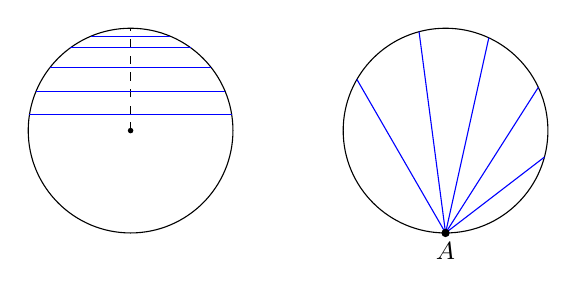
\begin{tikzpicture}[scale=1.0]
		\draw (0,0) circle (1.3);
		\draw[dashed] (0,0) -- (0,1.3);
		\foreach \y in {0.2, 0.5, 0.8, 1.05, 1.2}
			\draw[color=blue] ({-sqrt(1.69 - \y*\y)}, \y) -- ({sqrt(1.69 - \y*\y)}, \y);
		\fill (0,0) circle (1pt);
		\begin{scope}[xshift=4cm]
			\draw (0,0) circle (1.3);
			\foreach \a in {150, 105, 65, 25, -15}
				\draw[color=blue] (-90:1.3) -- (\a:1.3);
			\fill (-90:1.3) circle (1.5pt);
			\node[below, font=\small] at (-90:1.3) {$A$};
		\end{scope}
	\end{tikzpicture}
	\end{center}
	Two perfectly reasonable readings of `a random chord'; two different answers. There is no paradox once we accept that the two procedures generate genuinely different distributions on chords -- the lesson is that in continuous settings, the model must be specified, not assumed.
\end{example}

\subsection{Buffon's Needle}

Our second classic has a happier punchline: a probabilistic experiment that computes $\pi$.

\begin{example}[Buffon's Needle]
	A floor is ruled with parallel lines a distance $L$ apart, and a needle of length $\ell \leq L$ is dropped on it at random. What is the probability that the needle crosses a line?
	\begin{center}
	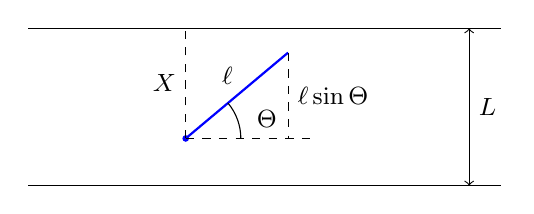
\begin{tikzpicture}[scale=1.0]
		\draw (0,0) -- (6,0);
		\draw (0,2) -- (6,2);
		\draw[<->] (5.6,0) -- (5.6,2);
		\node[right, font=\small] at (5.6,1) {$L$};
		\draw[thick, color=blue] (2,0.6) -- (3.3,1.69);
		\fill[blue] (2,0.6) circle (1.2pt);
		\node[above left, font=\small] at (2.72,1.16) {$\ell$};
		\draw[dashed] (2,0.6) -- (2,2);
		\node[left, font=\small] at (2,1.3) {$X$};
		\draw[dashed] (2,0.6) -- (3.6,0.6);
		\draw (2.7,0.6) arc (0:40:0.7);
		\node[font=\small] at (3.03,0.85) {$\Theta$};
		\draw[dashed] (3.3,1.69) -- (3.3,0.6);
		\node[right, font=\small] at (3.3,1.14) {$\ell\sin\Theta$};
	\end{tikzpicture}
	\end{center}

	We model the drop by two independent random variables: the distance $X \sim \mathrm{U}[0, L]$ from the needle's lower end\footnote{Lower in the direction perpendicular to the lines, say.} to the nearest line above it, and the angle $\Theta \sim \mathrm{U}[0, \pi]$ the needle makes with the lines. The needle crosses a line precisely when $\ell\sin\Theta \geq X$, so
	$$
	p = \PP(X \leq \ell\sin\Theta) = \int_0^{\pi}\!\!\int_0^{L} \frac{1}{\pi L}\,\ii_{\{x \leq \ell\sin\theta\}} \dd x \dd\theta = \frac{1}{\pi L}\int_0^{\pi} \ell \sin\theta \dd\theta = \frac{2\ell}{\pi L}.
	$$
\end{example}

Since $\pi = 2\ell/pL$, we can \emph{estimate} $\pi$ by dropping $n$ needles, letting $\hat{p}_n$ be the observed proportion of crossings, and computing $\hat\pi_n = 2\ell/\hat{p}_n L$. How good is this? This is exactly the sampling problem from the previous section: by the CLT,
$$
\hat p_n \approx p + \sqrt{\frac{p(1-p)}{n}}\,Z, \quad Z \sim N(0,1),
$$
and applying the first-order Taylor expansion $f(\hat p_n) \approx f(p) + (\hat p_n - p)f'(p)$ to $f(x) = 2\ell/xL$ (which has $f'(p) = -\pi/p$),
$$
\hat\pi_n - \pi \approx -\pi\sqrt{\frac{1 - p}{pn}}\, Z.
$$
Asking for $|\hat\pi_n - \pi| \leq 0.001$ with probability $0.99$ and consulting tables ($\PP(|Z| \leq 2.58) = 0.99$) leads to $n$ of order $10^7$ drops. As numerical integration schemes go, this one converges \emph{very} slowly -- the $1/\sqrt{n}$ error decay of averages is no match for even basic quadrature -- but as a party trick it remains unbeatable.

\subsection{Simulating Random Variables}

Suppose we have a source of uniform randomness -- a computer's random number generator handing us independent $\mathrm{U}[0, 1]$ variables -- and we want to manufacture a random variable with some other prescribed distribution $F$. There is a beautifully simple recipe: feed the uniform through the inverse of $F$.

\begin{theorem}[Inverse Transform Sampling]
	Let $F$ be a continuous, strictly increasing distribution function, and let $U \sim \mathrm{U}[0, 1]$. Then
	$$
	X = F^{-1}(U) \quad \text{has distribution function } F.
	$$
\end{theorem}
\begin{proof}
	Since $F$ is increasing, $F^{-1}(U) \leq x \iff U \leq F(x)$, and so
	$$
	\PP(X \leq x) = \PP(U \leq F(x)) = F(x),
	$$
	as $F(x) \in [0, 1]$ and $U$ is uniform.
\end{proof}

The intuition: $F^{-1}(p)$ is the value that the distribution places probability $p$ below, so sampling a uniform `probability level' and inverting produces values with exactly the right frequencies.

\begin{example}
	Taking $F(x) = 1 - e^{-x}$, we get that if $U \sim \mathrm{U}[0,1]$ then $F^{-1}(U) = -\log(1 - U)$ is $\mathrm{Exp}(1)$ -- and since $1 - U$ is also uniform, more simply $-\log U \sim \mathrm{Exp}(1)$. Similarly, the Box-Muller observation from our polar coordinates example gives a normal sampler: with independent $U_1, U_2 \sim \mathrm{U}[0,1]$, the variables
	$$
	X = \sqrt{-2\log U_1}\,\cos(2\pi U_2), \qquad Y = \sqrt{-2\log U_1}\,\sin(2\pi U_2)
	$$
	are independent standard normals, since $\sqrt{-2\log U_1}$ has the density $re^{-r^2/2}$ of the Gaussian radius and $2\pi U_2$ is a uniform angle.
\end{example}

Inverse transform sampling needs a computable $F^{-1}$, which is often unavailable (already for the normal distribution one has to work around it, as above). Our final method needs only the density -- and the willingness to throw samples away.

\begin{theorem}[Rejection Sampling]
	Let $A \subseteq [0, 1]^d$ have volume $|A| > 0$, and let $U_1, U_2, \dots$ be independent uniform points in $[0,1]^d$. Let $N = \min\{n \geq 1 : U_n \in A\}$. Then $U_N$ is uniformly distributed on $A$.
\end{theorem}
\begin{proof}
	Let $B \subseteq [0,1]^d$. Splitting according to the value of $N$ and using independence,
	\begin{align*}
		\PP(U_N \in B) &= \sum_{n = 1}^{\infty} \PP(U_n \in A \cap B,\ U_{n-1} \notin A, \dots, U_1 \notin A) \\
		&= \sum_{n = 1}^{\infty} |A \cap B| \, (1 - |A|)^{n - 1} = \frac{|A \cap B|}{|A|},
	\end{align*}
	summing the geometric series. This is exactly the uniform distribution on $A$.
\end{proof}

To simulate a random variable on $[0,1]^{d-1}$ with a bounded density $f \leq \lambda$, we apply this with the region \emph{under the (scaled) graph of $f$}:
$$
A = \left\{(x_1, \dots, x_d) \in [0,1]^d : x_d \leq \frac{f(x_1, \dots, x_{d-1})}{\lambda}\right\}.
$$
Generate a uniform point of $A$ by rejection, and keep only its first $d - 1$ coordinates $X$. For any $B \subseteq [0,1]^{d - 1}$, integrating out the last coordinate gives
$$
\PP(X \in B) = \frac{|(B \times [0,1]) \cap A|}{|A|} = \frac{\frac{1}{\lambda}\int_B f(x)\dd x}{\frac{1}{\lambda}\int f(x) \dd x} = \int_B f(x)\dd x,
$$
so $X$ has density $f$, as desired. In words: throw uniform darts at the box, keep the ones landing under the graph of the density, and read off their horizontal coordinates. It is a fittingly concrete note on which to end -- the abstract machinery of densities, built up from three axioms about measures, cashing out as instructions you could implement in ten lines of code.


